\section{Mesh Generation and Management}

Given a mesh, all the mesh support needed to run M3D-C$^{1}$ is provided by PUMI (Parallel Unstructured Mesh Infrastructure) developed at RPI Scientific Computation Research Center (SCOREC). The PUMI is used to manage the mesh information as it is processed within the M3D-C$^{1}$ code. PUMI is a freely available open source software. For more information on how to get and install, visit \href{http://www.scorec.rpi.edu/pumi}{http://www.scorec.rpi.edu/pumi}.

The generation of M3D-C$^{1}$ meshes for Tokamak geometries using the M3D-C$^{1}$ mesh generation program involves both PUMI and Simmetrix mesh generation software. Simmetrix is commercial software which provides a set of tools and libraries for engineering simulation. As Simmetrix runs only with a valid license, any M3D-C$^{1}$ user who wants to install his/her own version of the M3D-C$^{1}$ mesh generation program should contact Simmetrix to purchase its license. For more information on Simmetrix, visit \href{http://simmetrix.com}{http://simmetrix.com}. {M3D-1}$^{1}$ users with accounts on \texttt{PPPL Portal} or \texttt{Princeton Stellar} are allowed to run M3D-C$^{1}$ mesh mesh generation programs on those systems.
%In order to obtain an account on those two machines, contact M3D-C$^{1}$ group (\href{mailto:jardin@pppl.gov}{jardin@pppl.gov}).

Note that Simmetrix software is not required to run a M3D-C$^{1}$ simulation. Running a M3D-C$^{1}$ simulation using a mesh generated by a different mesh generator requires the development of a tool that creates PUMI readable model and mesh files with M3D-C$^{1}$ related control information required as the M3D-C$^{1}$ input. For more information, contact RPI SCOREC (\href{mailto:shephard@rpi.edu}{shephard@rpi.edu}).
\newline

With respect to the mesh support, there are a number of files involved with housing the geometry and mesh information. First, the model file extensions are the following
\begin{itemize}
\item \texttt{.smd}: Simmetrix-readable binary format model file  
\newline  The model generated with Simmetrix is saved in this format.
\item \texttt{.dmg}: PUMI-readable binary format model file
\newline	The model generated from PUMI mesh
\item	\texttt{.txt}: M3D-C$^{1}$-readable ascii format model file 
\newline	The model is generated from mesh generation tool (See Section~\ref{ch:mesh-gen})
\end{itemize}

Second, the mesh file extensions are the following.
\begin{itemize}
\item	\texttt{.sms}: Simmetrix-readable binary format mesh file
\begin{itemize}
\item	The mesh generated with Simmetrix is saved in this format.
\item	If a mesh is serial (1-part), the mesh file doesn't have a number before the extension
\item	If a mesh is distributed (\texttt{P}-part, P$>$1), the mesh file has a number before the extension to represent the global part ID.
\end{itemize}
\item	\texttt{.smb}: PUMI-readable binary format mesh file
\begin{itemize}
\item	This format is used in M3D-C$^{1}$ to import/export a mesh
\item	No matter if a mesh is serial (1-part) or distributed (\texttt{P}-part, P$>$1), the mesh file has a number before the extension to represent the global part ID.
\end{itemize}
\item \texttt{.vtu/pvtu}: binary format mesh file for visualization with Paraview. For more information, visit \href{http://paraview.org}{http://paraview.org}.
\end{itemize}

An overview of the Model/Mesh requirements for the M3D-C$^{1}$ mesh generation process are as follows:
\begin{itemize}
\item	The model and mesh shall be generated as described in Section~\ref{ch:mesh-gen}.
\item	The mesh file must be PUMI-readable \texttt{.smb} file. Note that a mesh file name contains a number before the extension (.smb) to denote a global part ID.
\item	The model and mesh file must be present in the work directory
\item	The name of model and mesh file must be specified in \texttt{C1input} file in the work directory
\begin{itemize}
\item	mesh\_model = model\_file
\item	mesh\_filename = mesh\_file.smb (NOTE: do not specify a number before the file extension)
\end{itemize}
\item In a 2D run with \texttt{P} processes, there should be \texttt{P} mesh files with part ID from \texttt{0} to \texttt{P-1}
\item	In a 3D run with \texttt{P$\times$N} processes where 2D mesh is distributed to \texttt{P} parts, 
\begin{itemize}
\item	there should be \texttt{P} mesh files with part ID from \texttt{0} to \texttt{P-1}
\item	in \texttt{C1input} file, specify \texttt{nplanes} to \texttt{N} (e.g. nplanes=8), where \texttt{nplanes} describes how many 2D mesh copies to be loaded
\item	the M3D-C$^{1}$ code should be compiled with options \texttt{"3D=1, MAX\_PTS=60"}.
\end{itemize}
\end{itemize}

The rest of this section is organized as follows: Section \ref{ch:mesh-gen} describes a mesh generation program \texttt{m3dc1\_meshgen}. Section \ref{ch:mfm-gen} describes a mesh generation program \texttt{m3dc1\_mfmgen}. Section \ref{ch:polar-gen} describes a mesh generation program \texttt{polar\_meshgen}. Section \ref{ch:mesh-ptn} presents a mesh partitioning program \texttt{"split\_smb"} and \texttt{"collapse"} which changes the number of parts of the mesh. For how to visualize a mesh with \texttt{Paraview}, see Appendix~\ref{ch:app-paraview}.

%%%%%%%%%%%%%%%%%%%%%%%%%%%%%%%%%%%%%%%%%
\subsection{m3dc1\_meshgen}
\label{ch:mesh-gen}
%%%%%%%%%%%%%%%%%%%%%%%%%%%%%%%%%%%%%%%%%

\texttt{m3dc1\_meshgen} requires an ascii input file of arbitrary name that contains the following parameters.

\begin{itemize}
\item modelType: 0, 1, 2, 3, or 4
\begin{itemize}
\item Type 0: a parameterized vacuum region defined by five doubles for analytic expression. 
For five doubles $X_0$   $X_1$   $X_2$   $Z_0$   $Z_1$, vacuum boundary is defined by 
\begin{equation}
X = X_0 + X_1 cos(\theta + X_2*sin(\theta))
\end{equation}
\begin{equation}
Z =  Z_0 + Z_1 sin(\theta)
\end{equation}
\item	Type 1: a vacuum region defined by piece-wise linear points
\item	Type 2: a vacuum region defined by piece-wise polynomials
\item	Type 3: spline-fitted 3-region model (plasma, wall and vacuum)
\item	Type 4: spline-fitted 3-region model (plasma, wall, and vacuum) with inner \& outer boundary points to set resistive wall
\end{itemize}

\item reorder: if 1, reorder PUMI mesh based on adjacency (default: 0) and generate vtk folders for mesh visualization. The mesh before and after reodering is saved in \texttt{original-mesh.vtk} and \texttt{reordered-mesh.vtk}, respectively. Note that the element order of Simmetrix mesh is not affected.
\item inFile: (modelType 0) not required
(modelType 1 and 2) geometry file describing the vacuum (modelType 3 and 4) geometry file describing the inner plasma wall
\item bdryFile: (modelType 0-3) not required
 (modelType 4) geometry file describing the outer plasma wall
\item outFile: output file name to save model and mesh
\item meshSize: relative mesh size for each region (default 0.05)
\newline
	for modelType 3, set three doubles for plasma, resistive, vacuum, respectively
\item useVacuumParams: for modelType 0 or 3, if 1, use parameterized vacuum wall (default 0)
\item vacuumParams: five doubles to describe parameterized vacuum wall. Required if useVacuumParams=1.
\item adjustVacuumParams: for modelType 0 or 3, if 1, multiply coordinates and parametric values of nodes on vacuum wall by vacuumFactor. Valid only if useVacuumParams=1 (default 0)
\item vacuumFactor: for modelType 0 or 3, an optional double value used to multiply coordinates and parametric values of nodes on vacuum wall when adjustVacuumParams=1. Valid only if adjustVacuumParams=1 (default 2$\times$PI)
\item numVacuumPts: optional \# interpolation points on parameterized vacuum wall. Valid only if useVacuumParams=1 (default 20)
\item meshGradationRate: for modelType 3 or 4, optional mesh gradation rate (default: 0.3). This value should be greater than or equal to 0.3. Otherwise the mesh will be fine everywhere.
\item resistive-width: for modelType 3, the width of resistive wall. If resistive-width=0, only plasma region is created (default 0.02)
\item plasma-offsetX: for modelType 3, the offset in x direction to the left (default 0.0)
\item plasma-offsetY: for modelType 3, the offset in y direction to the bottom (default 0.0)
\item vacuum-width: for modelType 3 or 4, the width of vacuum region (default 2.5)
\item vacuum-height: for modelType 3 or 4, the height of vacuum region (default 4.0) 
\end{itemize}

Locate input parameter file and all files listed as bdryFile (if applicable) in the work folder and do \texttt{m3dc1\_meshgen input\_param\_file}, then the following output will be generated.

\begin{itemize}
\item The output model in three formats
  \begin{itemize}
  \item $M3D-C^1$-readable \texttt{.txt}
  \item Simmetrix-readable file \texttt{.smd} and
  \item PUMI-readable \texttt{.dmg}
    \begin{itemize}
    \item[$\triangleright$] For modelType 0-2, the model is saved in \texttt{outFile.*}
    \item[$\triangleright$] For modelType 3 with resistive width \texttt{R}, vacuum-width \texttt{W} and vacuum-height \texttt{H}, the model is saved in \texttt{outFile-R-W-H.*}.
    \item[$\triangleright$] For modelType 4 with vacuum-width \texttt{W} and vacuum-height \texttt{H}, the model is saved in \texttt{outFile-W-H.*}.
    \end{itemize}
  \end{itemize}
\item The output mesh in three formats
  \begin{itemize}
  \item Simmetrix-readable\texttt{.sms}
  \item $M3D-C^1$/PUMI readable \texttt{.smb}
  \item Paraview
    \begin{itemize}
    \item[$\triangleright$] For modelType 0-2 with \# mesh faces \texttt{F},
      \begin{itemize}
      \item[-] if \texttt{F} $>$ 1000, the mesh is saved in \texttt{outFile-(F/1000).*}
      \item[-] if \texttt{F} $<$ 1000, the mesh is saved in \texttt{outFile-F.*}
      \end{itemize}
    \item[$\triangleright$] For modelType 3 with \# mesh faces \texttt{F}, resistive width \texttt{R}, vacuum-width \texttt{W}, vacuum-height \texttt{H},
      \begin{itemize}
      \item[-] if \texttt{F} $>$ 1000, the mesh is saved in \texttt{outFile-R-W-H-(F/1000).*}
      \item[-] if \texttt{F} $<$ 1000, the mesh is saved in \texttt{outFile-R-W-H-F.*}
      \end{itemize}
    \item[$\triangleright$] For modelType 4 with \# mesh faces \texttt{F}, vacuum-width \texttt{W} and vacuum-height \texttt{H},
      \begin{itemize}
      \item[-] if \texttt{F} $>$ 1000, the mesh is saved in \texttt{outFile-W-H-(F/1000).*}
      \item[-] if \texttt{F} $<$ 1000, the mesh is saved in \texttt{outFile-W-H-F.*}
      \end{itemize}
    \end{itemize}
  \end{itemize}
\end{itemize}

%%%%%%%%%%%%%%%%%%%%%%%%%%%%%%%%%%%%%%%%%
\subsubsection{Type 0 (parameterized vacuum)}
%%%%%%%%%%%%%%%%%%%%%%%%%%%%%%%%%%%%%%%%%

\begin{figure}
\centering
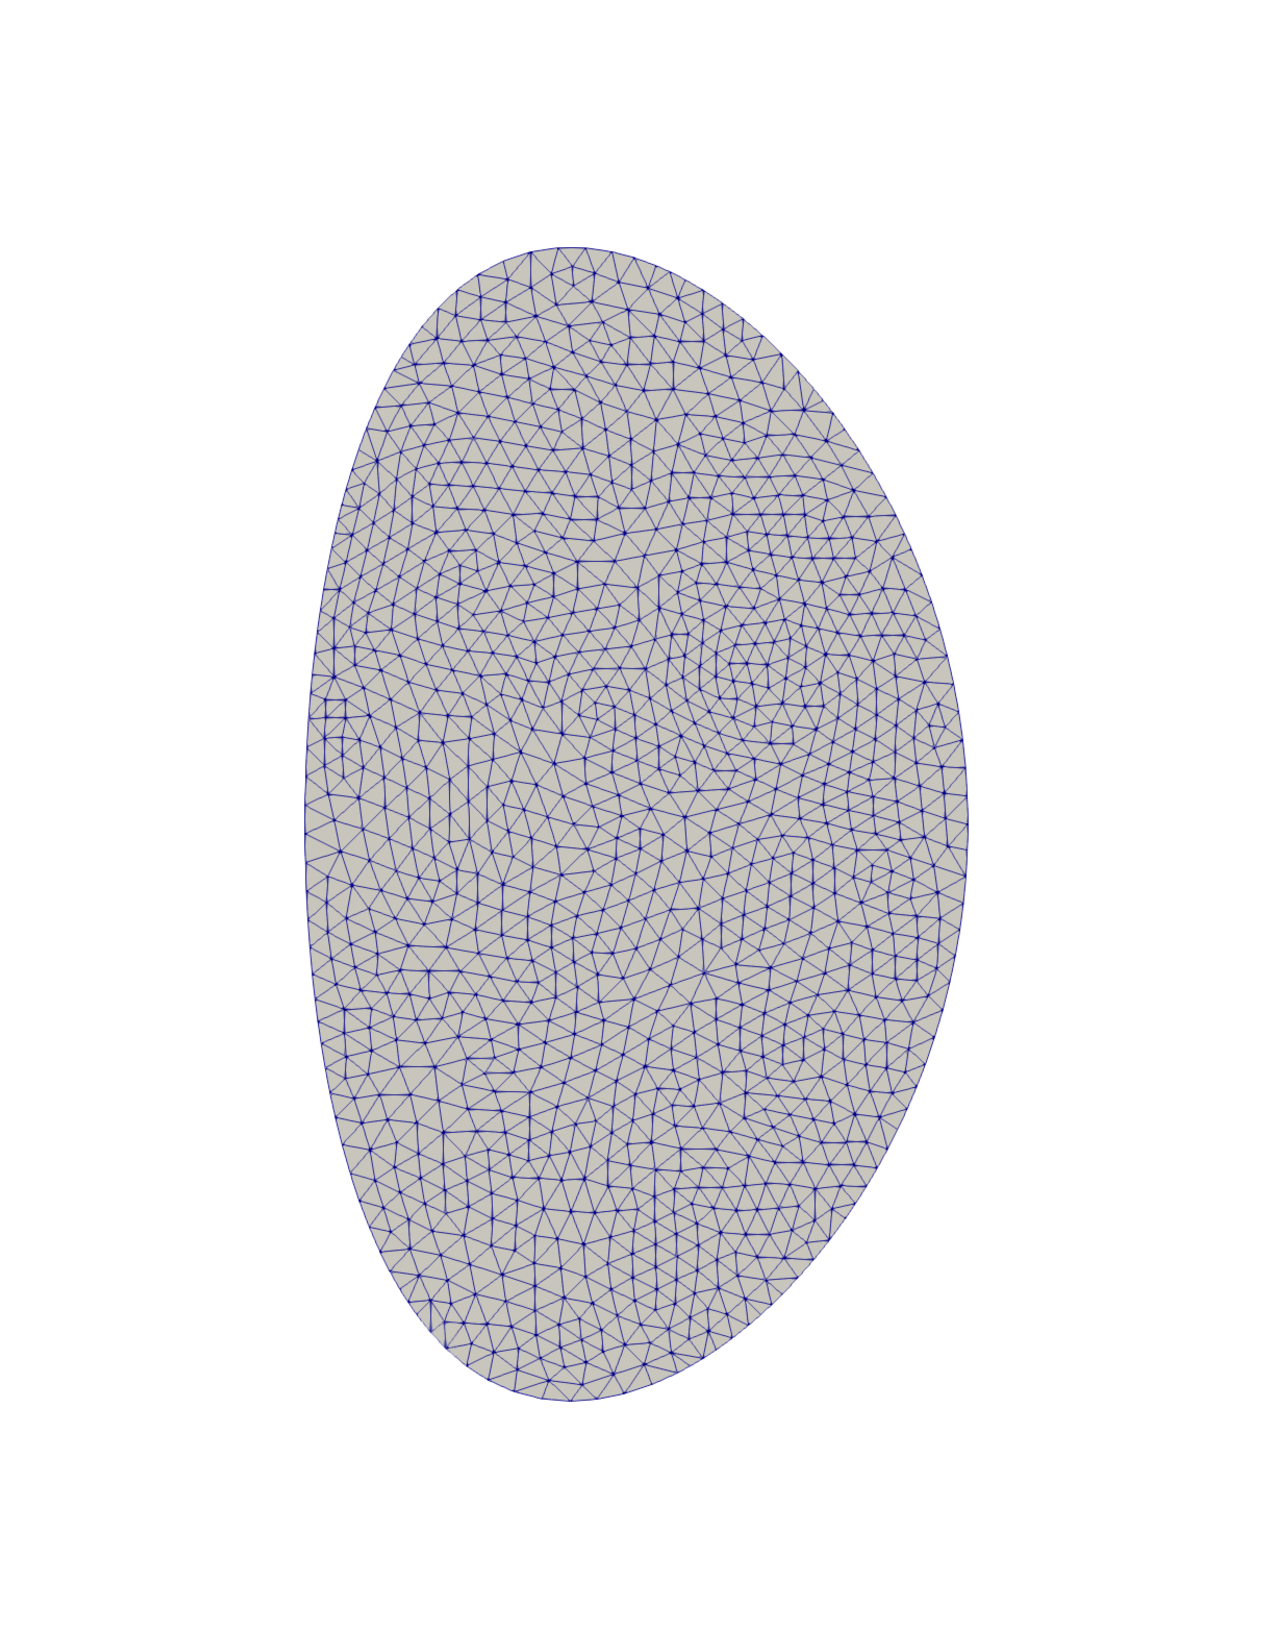
\includegraphics[width=3in]{./figures/meshgen-type0.pdf}
\caption[Mesh with vacuum region defined by five parameters for analytic expression]
{A mesh with vacuum region defined by five parameters for analytic expression}
\label{fig:meshgen-type0}
\end{figure}

The figure~\ref{fig:meshgen-type0} illustrates a mesh generated by the following input file.

\begin{verbatim}
modelType 0
outFile analytic 
meshSize 0.04

useVacuumParams 1
vacuumParams 1.65908 0.46 0.2 -0.02504 0.8
numVacuumPts 20

adjustVacuumParams 0
vacuumFactor  6.28319
\end{verbatim}

\begin{figure}
\centering
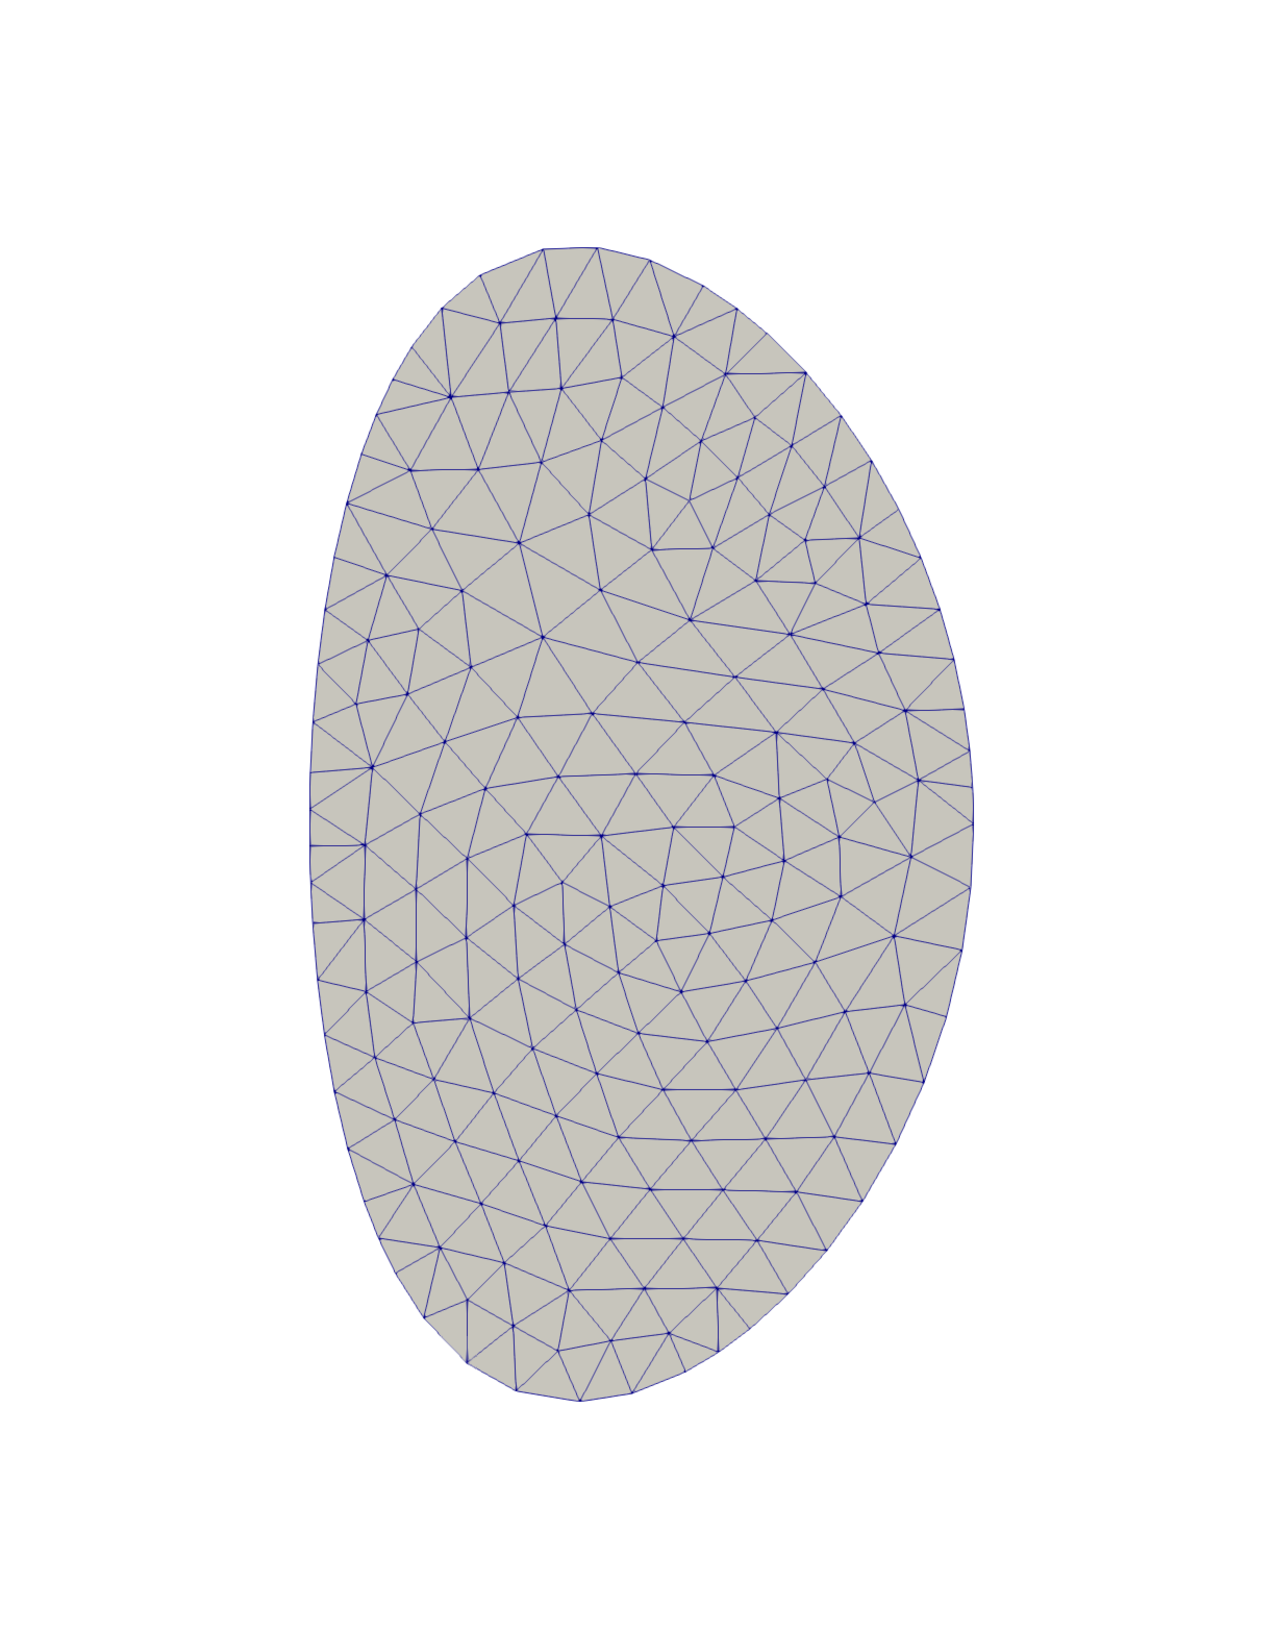
\includegraphics[width=3in]{./figures/meshgen-type0-ms.pdf}
\caption[Mesh generated with vacuum region parameters and mesh size 0.1]
{A mesh generated with vacuum region parameters and mesh size 0.1}
\label{fig:meshgen-type0-ms}
\end{figure}

The figure~\ref{fig:meshgen-type0-ms} illustrates a mesh generated with the same vacuum region parameters and a higher mesh size value.

%%%%%%%%%%%%%%%%%%%%%%%%%%%%%%%%%%%%%%%%%
\subsubsection{Type 2 (piece-wise polynomial vacuum)}
%%%%%%%%%%%%%%%%%%%%%%%%%%%%%%%%%%%%%%%%%

\begin{figure}
\centering
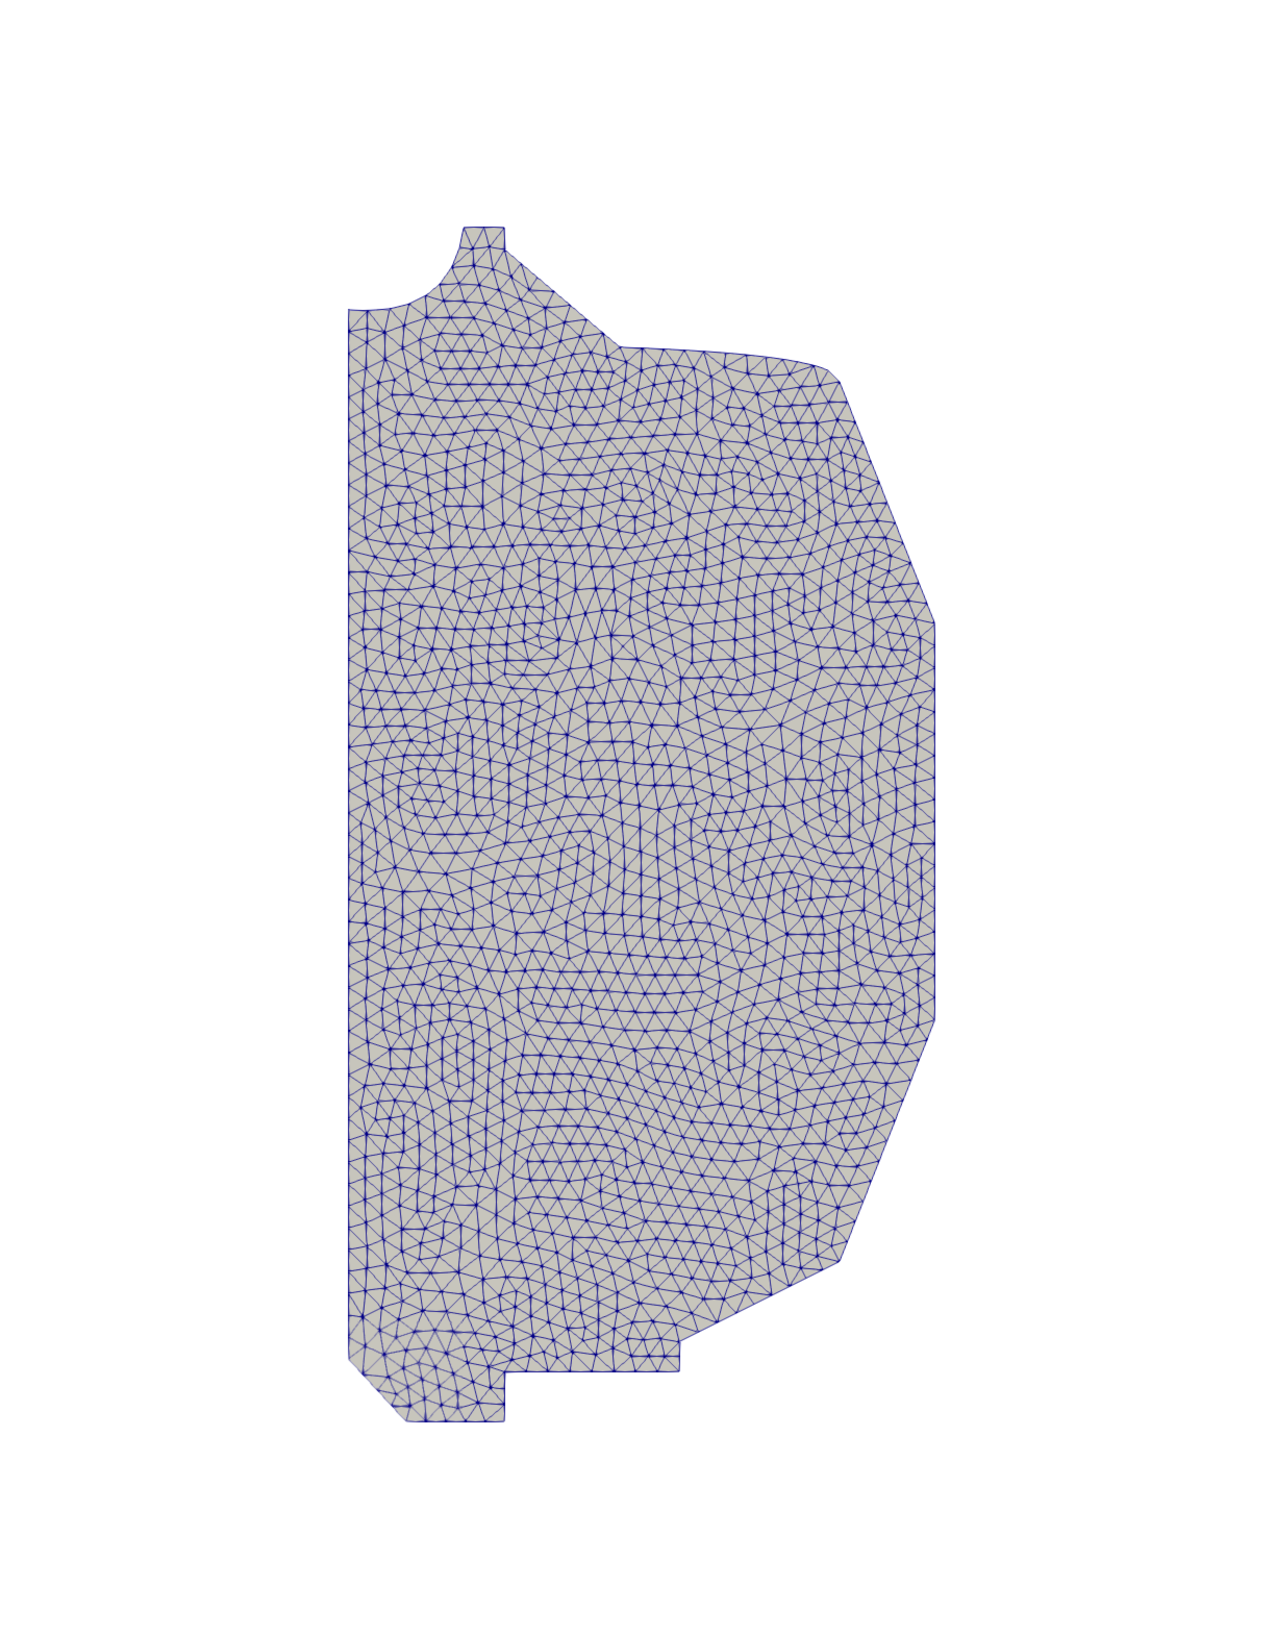
\includegraphics[width=3in]{./figures/meshgen-type2.pdf}
\caption[Mesh with vacuum region defined by piece-wise polynomials]
{A mesh with vacuum region defined by piece-wise polynomials}
\label{fig:meshgen-type2}
\end{figure}

The figure~\ref{fig:meshgen-type2} illustrates a mesh generated by the following input file. The vacuum region's geometry information is defined by piece-wise polynomials and stored in the file \texttt{in-poly}. 

\begin{verbatim}
modelType 2
inFile in-poly
outFile poly
\end{verbatim}

The vacuum region's geometry information is defined by piece-wise polynomials and stored in the file \texttt{in-poly} and the example file can be found in 
\newline\newline
\texttt{/p/tsc/m3dc1/lib/SCORECLib/rhel7/intel2019u3-openmpi4.0.3/16.0-220226/bin}.

%%%%%%%%%%%%%%%%%%%%%%%%%%%%%%%%%%%%%%%%%
\subsubsection{Type 3 (three-regions with inner wall points)}
%%%%%%%%%%%%%%%%%%%%%%%%%%%%%%%%%%%%%%%%%
With the model type 3, a geometric model consists of three model faces where each represents plasma region, resistive region and vacuum region, respectively. An ascii file name which describes inner plasma wall boundary has to be provied with the parameter \texttt{inFile}.

\begin{figure}
\centering
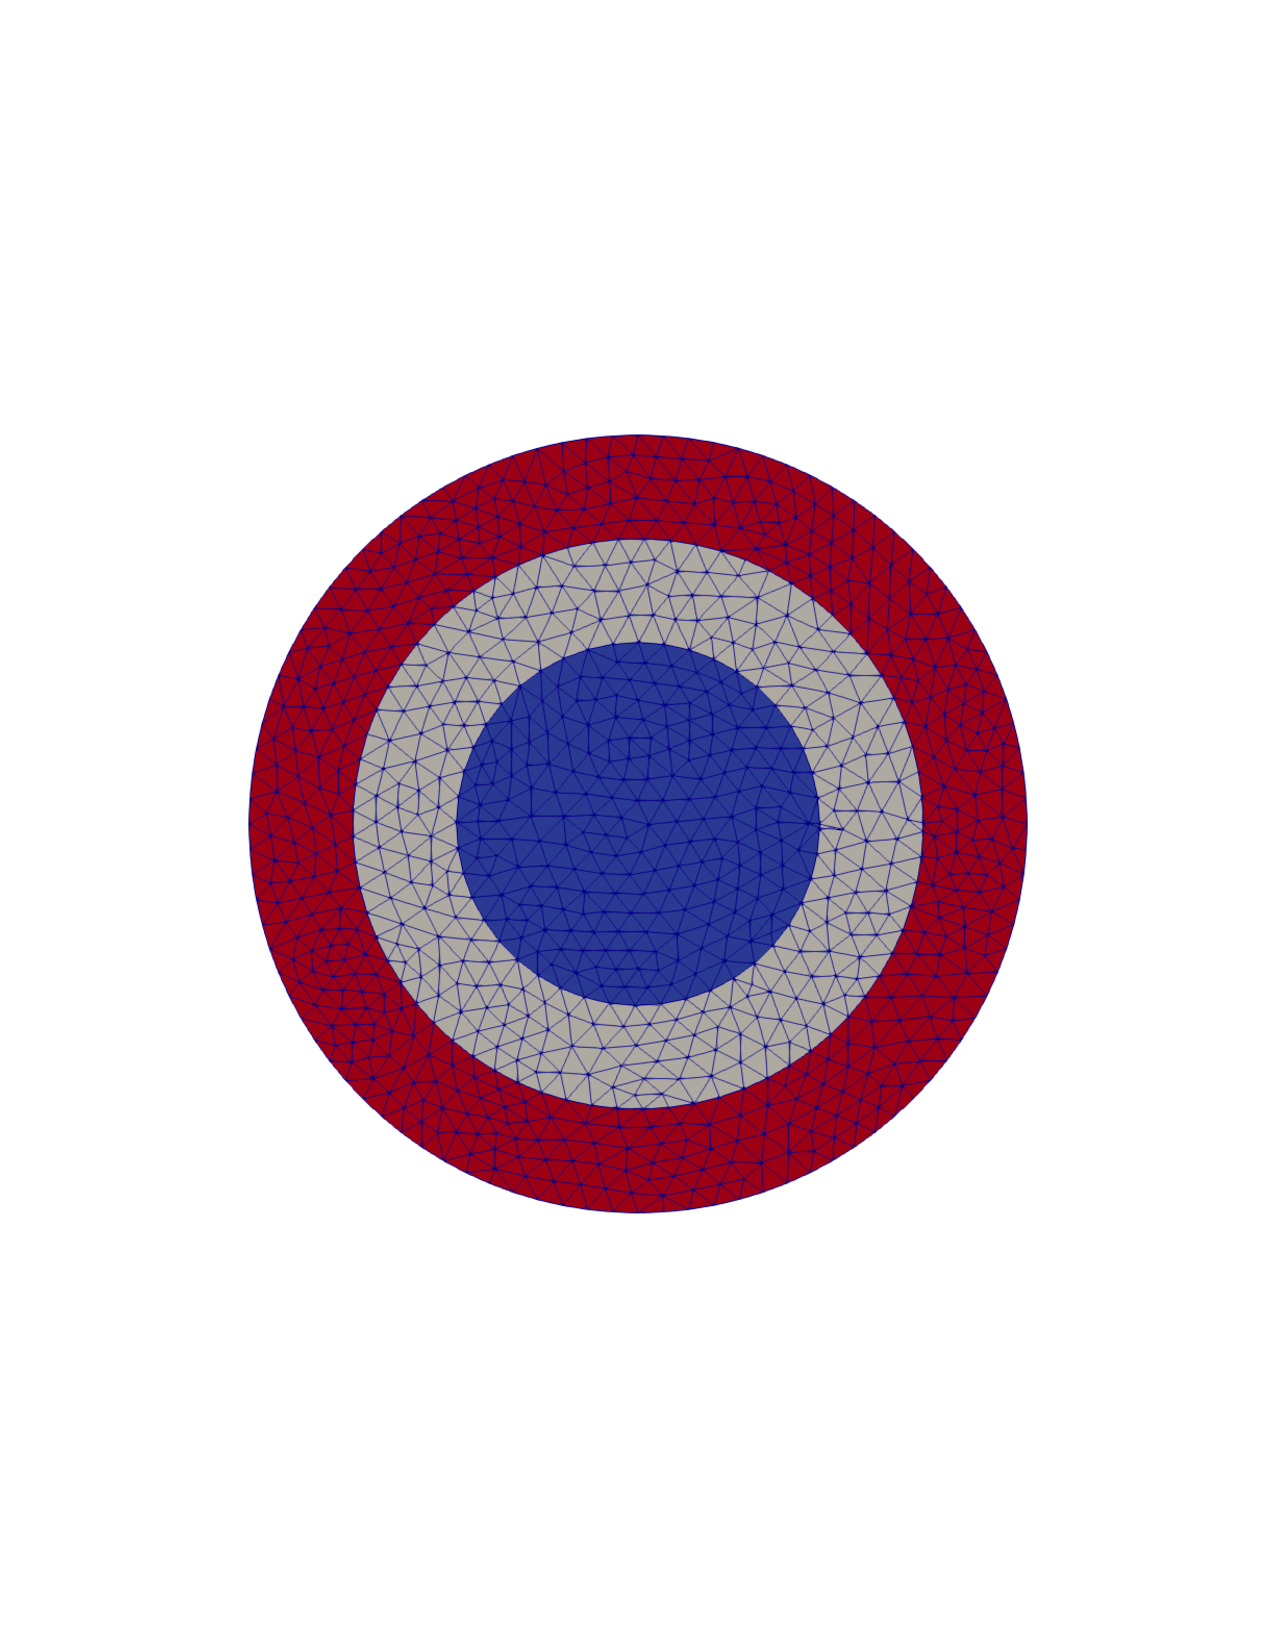
\includegraphics[width=3in]{./figures/meshgen-type3.pdf}
\caption[Mesh with spline-fitted 3-region model]
{A mesh with spline-fitted 3-region model}
\label{fig:meshgen-type3}
\end{figure}

The figure~\ref{fig:meshgen-type3} illustrates a mesh generated by the following input file. In the figure, geometric model faces are different colored.

\begin{verbatim}
modelType 3
inFile in-circle
outFile circle
meshSize 0.1 0.5 0.1
useVacuumParams 1
adjustVacuumParams 1
vacuumParams 5.0 1.5 0.0 0.0 1.5
numVacuumPts 20
meshGradationRate 0.4
resistive-width 0.4
\end{verbatim}

The example files \texttt{circle-input} and \texttt{in-circle} can be found in
\newline\newline
\texttt{/p/tsc/m3dc1/lib/SCORECLib/rhel7/intel2019u3-openmpi4.0.3/16.0-220226/bin}.

%%%%%%%%%%%%%%%%%%%%%%%%%%%%%%%%%%%%%%%%%
\subsubsection{Type 4 (three-regions with inner $\&$ outer wall points)}
%%%%%%%%%%%%%%%%%%%%%%%%%%%%%%%%%%%%%%%%%

With the model type 4, a geometric model consists of three model faces where each represents plasma region, resistive region and vacuum region, respectively.  The parameter \texttt{inFile} denotes a file name that contains inner plasma wall boundary. The parameter \texttt{bdryFile} denotes a file name that contains resistive wall boundary.

\begin{figure}
\centering
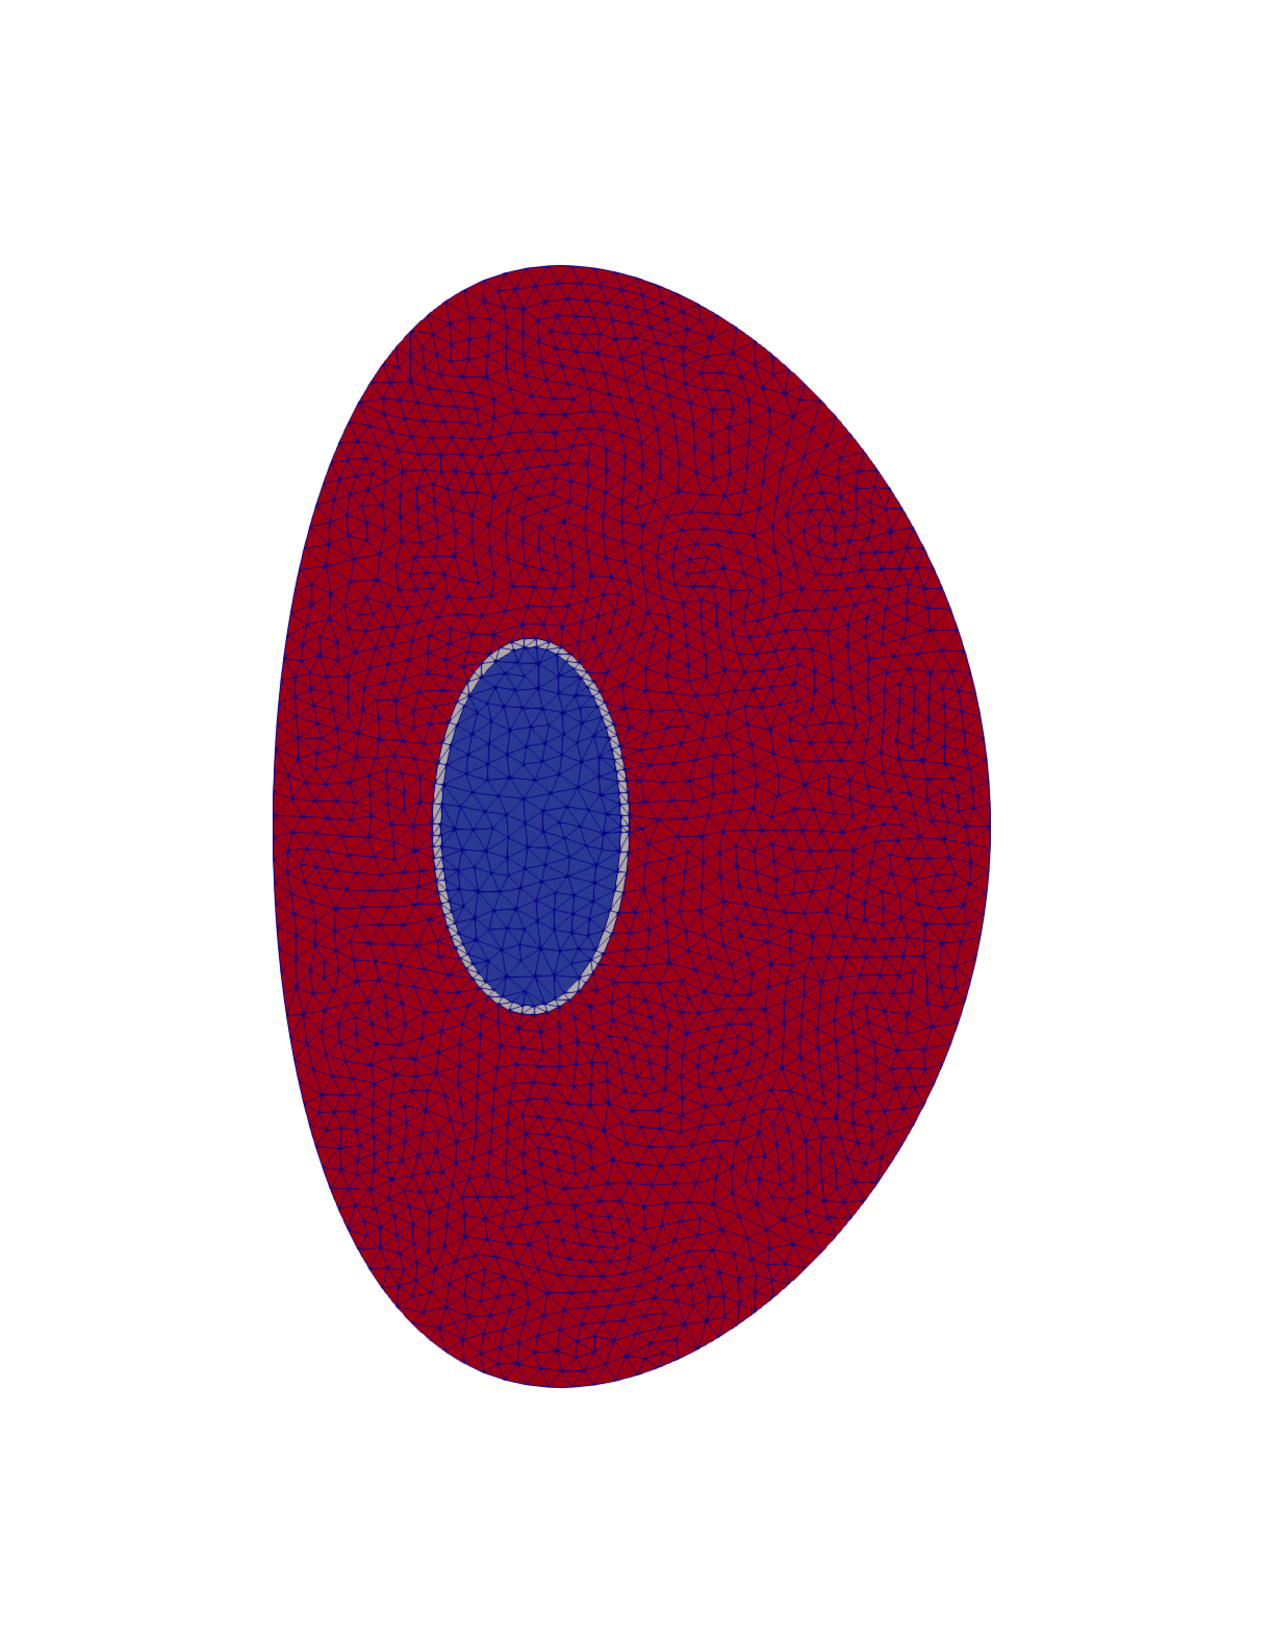
\includegraphics[width=3in]{./figures/meshgen-type4.pdf}
\caption[Mesh with inner $\&$ outer plasma wall boundary points]
{A mesh with inner $\&$ outer plama wall boundary points}
\label{fig:meshgen-type4}
\end{figure}

The figure~\ref{fig:meshgen-type4} illustrates a mesh generated by the following input file. In the figure, geometric model faces are different colored.

\begin{verbatim}
modelType 4
inFile inner_bdry.pts
bdryFile outer_bdry.pts
outFile iter
meshSize 0.7 0.5 0.7
useVacuumParams 1
adjustVacuumParams 1
vacuumParams 8.25 8.0 0.2 0.0 12.5
meshGradationRate 1
\end{verbatim}

The example files \texttt{bdry-input}, \texttt{inner\_bdry.pts} and \texttt{outer\_bdry.pts} can be found in
\newline\newline
\texttt{/p/tsc/m3dc1/lib/SCORECLib/rhel7/intel2019u3-openmpi4.0.3/16.0-220226/bin}.

%%%%%%%%%%%%%%%%%%%%%%%%%%%%%%%%%%%%%%%%%
\subsection{m3dc1\_mfmgen}
\label{ch:mfm-gen}
%%%%%%%%%%%%%%%%%%%%%%%%%%%%%%%%%%%%%%%%%

\texttt{m3dc1\_mfmgen} requires an ascii input file of arbitrary name that contains the following parameters.
The parameters can be in any order.

\begin{itemize}
\item numBdry: the number of boundary files defined by peice-wise linear points given for the construction of the loops (default: 0)
  \begin{itemize}
  \item Each boundary file corresponds to a loop in PUMI
  \item For \texttt{numBdry}=$N$, $N$ lines of \texttt{bdryFile} should be provided, $N \ge 0$
  \end{itemize}
\item bdryFile: For each boundary file, the user has to provide its file name followed by the unique loop ID and desired mesh size on the loop.
  \begin{itemize}
  \item Each boundary file corresponds to a loop in PUMI
  \item The unique ID can be an arbitrary integer defined by the user
  \item The unique ID is used with input parameter ``faceBdry" to specify the boundaries (loops) of model face
  \item For more than one boundary files (numBdry$>$1), the boundary files can be in any order
  \end{itemize}

\item useVacuum: A parameter to control the vacuum boundary
  \begin{itemize}
  \item The first number sets the mode of vacuum boundary and can be 0, 1 or 2. If 0, no vacuum boundary will be created. If 1, vacuum boundary will be created without user defined parameters. If 2, a parameterized vacuum boundary will be created by using the parameters defined in the parameter "vacuumParams".
  \item The second number is the desired unique loop ID for the vacuum loop
  \item  The third number defines the mesh size on the vacuum boundary
  \end{itemize}
\item vacuumParams: if ``useVacuum = 2", the user has to provide five doubles to define parameterized vacuum wall
\item numVacuumPts: if ``useVacuum = 2", \# interpolation points on parameterized vacuum wall (default=20)

\item thickWall: three integers and one double to control finite thickness wall
  \begin{itemize}
  \item The first number can either be 0 or 1. If it is set to 0, no finite thickness wall will be created. If it is set to 1, a finite thickness wall will be created
  \item The second number is the loop ID that will be offset for given thickness
  \item The third number is the desired unique loop ID for the new loop created from offsetting for the finite thickness wall
  \item The last number is the desired wall thickness
  \end{itemize} 

\item layeredMesh: two integers to create an extruded layeded mesh on the finite thickness wall
  \begin{itemize}
  \item The first integer is 0, no layered mesh will be created. If 1 (default), an extruded mesh with desired number of mesh layers will be created
  \item The second integer defines the number of mesh layers
  \end{itemize}

\item numFace: the number of geometric model faces in PUMI (default 1)
    \begin{itemize}
  \item Each geometric face corresponds to regions (e.g. plasma, resistive, vacuum) in M3DC1
  \item For \texttt{numFace}=$N$, $N$ lines of \texttt{faceBdry} should be provided, $N > 0$
  \end{itemize}
\item faceBdry: For each model face, the user has to provide the number of loops, loop ID(s), and desired mesh size
  \begin{itemize}
  \item The first number gives the total number of loops bounding the face
  \item the first number is followed by the loops IDs of the bounding loops. If number of loops = $n$, there should be $n$ loop ID
  \item The last number is the desired mesh size on the geometric face
    \end{itemize}

\item meshGradationRate: Global mesh gradation rate for the meshing. This parameter is optional and if not specified a default mesh gradation rate = 0.3 is used. This value should be greater than or equal to 0.3. Otherwise the mesh will be fine everywhere.
\item outFile: output file name to save model and mesh
\end{itemize}

Locate input parameter file and all files listed as bdryFile (if applicable) in the work folder and do \texttt{m3dc1\_mfmgen input\_param\_file}. The output files are the same as those of \texttt{m3dc1\_meshgen}.

%%%%%%%%%%%%%%%%%%%%%%%%%%%%%%%%%%%%%%%%%
\subsubsection{Mesh with parameterized vacuum wall}
%%%%%%%%%%%%%%%%%%%%%%%%%%%%%%%%%%%%%%%%%

This section presents a mesh created with a parameterized vacuum wall. This is equivalent to \texttt{Type 0} mesh of \texttt{m3dc1\_meshgen}.

\begin{verbatim}
numBdry 0
useVacuum 1 1 0.1
numFace 1
faceBdry 1 1 0.09
outFile analytic-0.09
\end{verbatim}

\begin{figure}
\centering
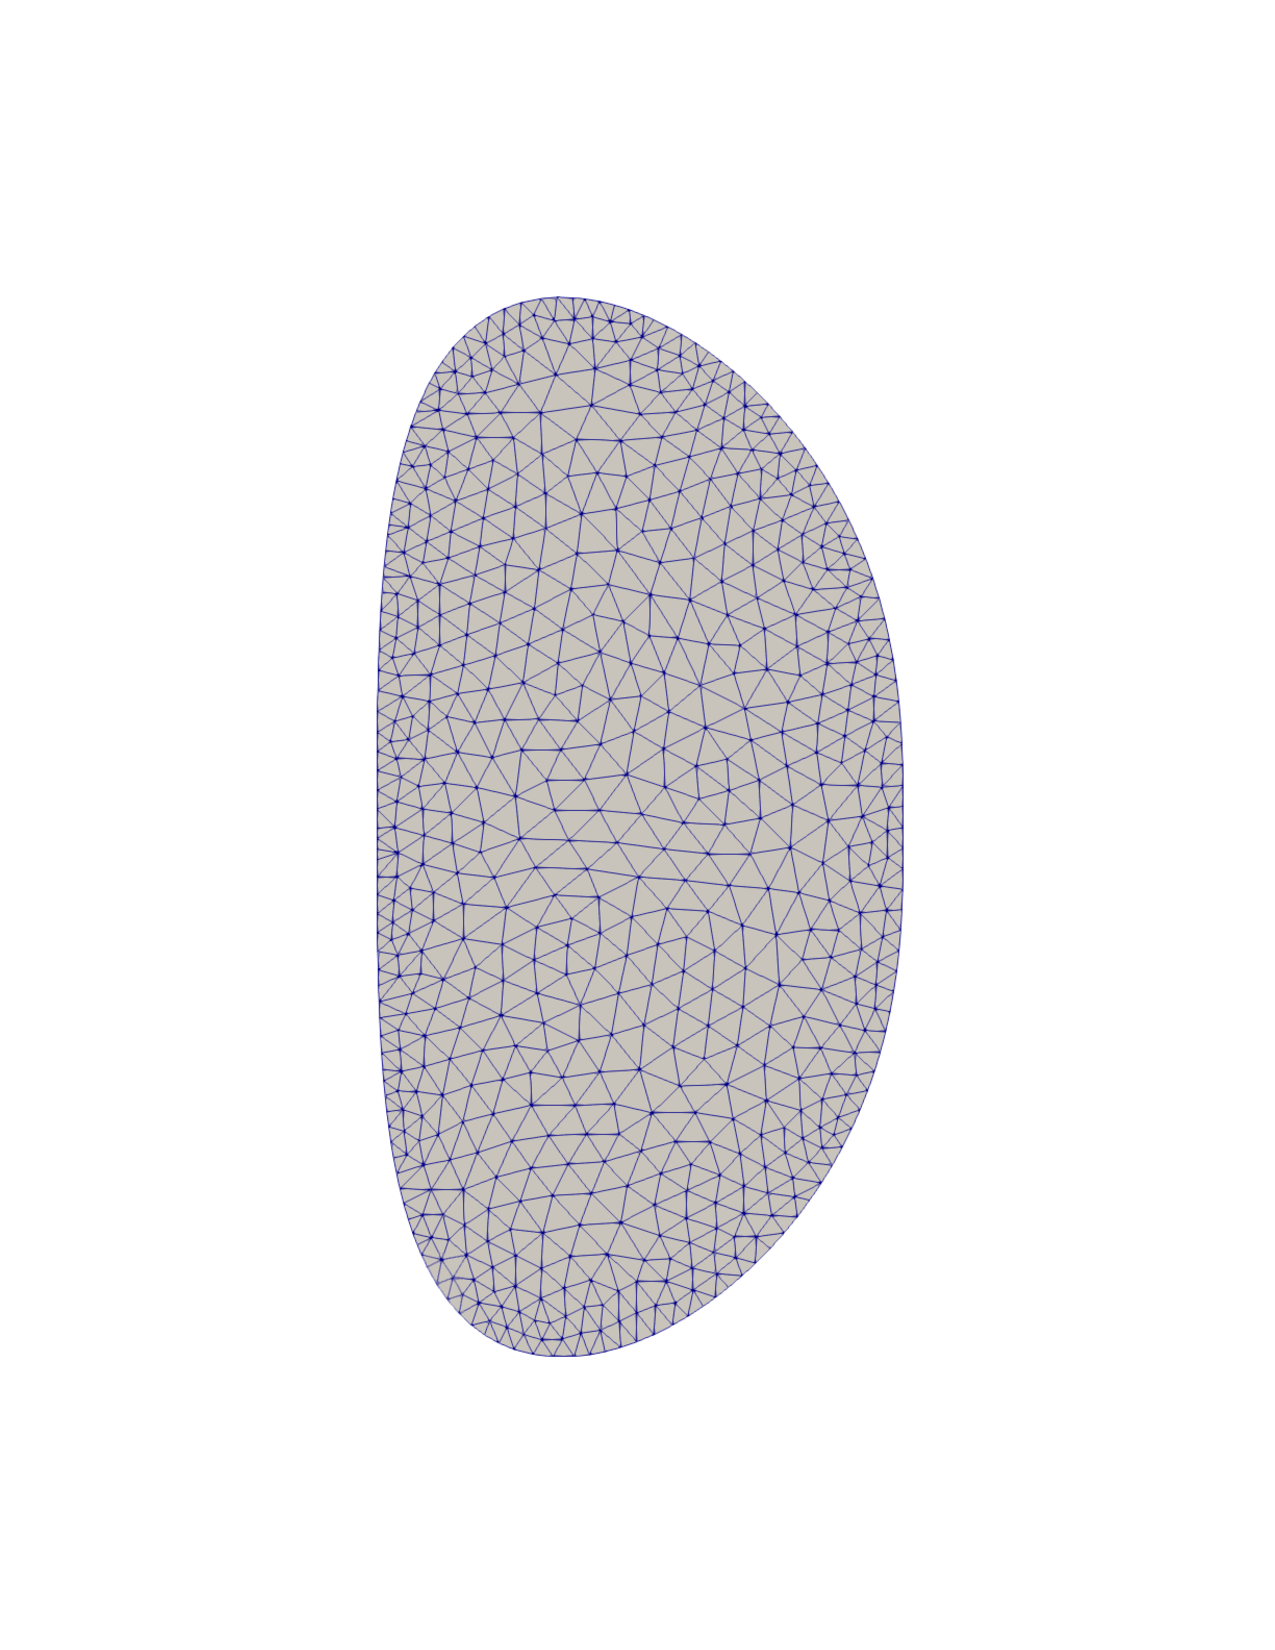
\includegraphics[width=3in]{./figures/meshgen-analytic-20pts-05.pdf}
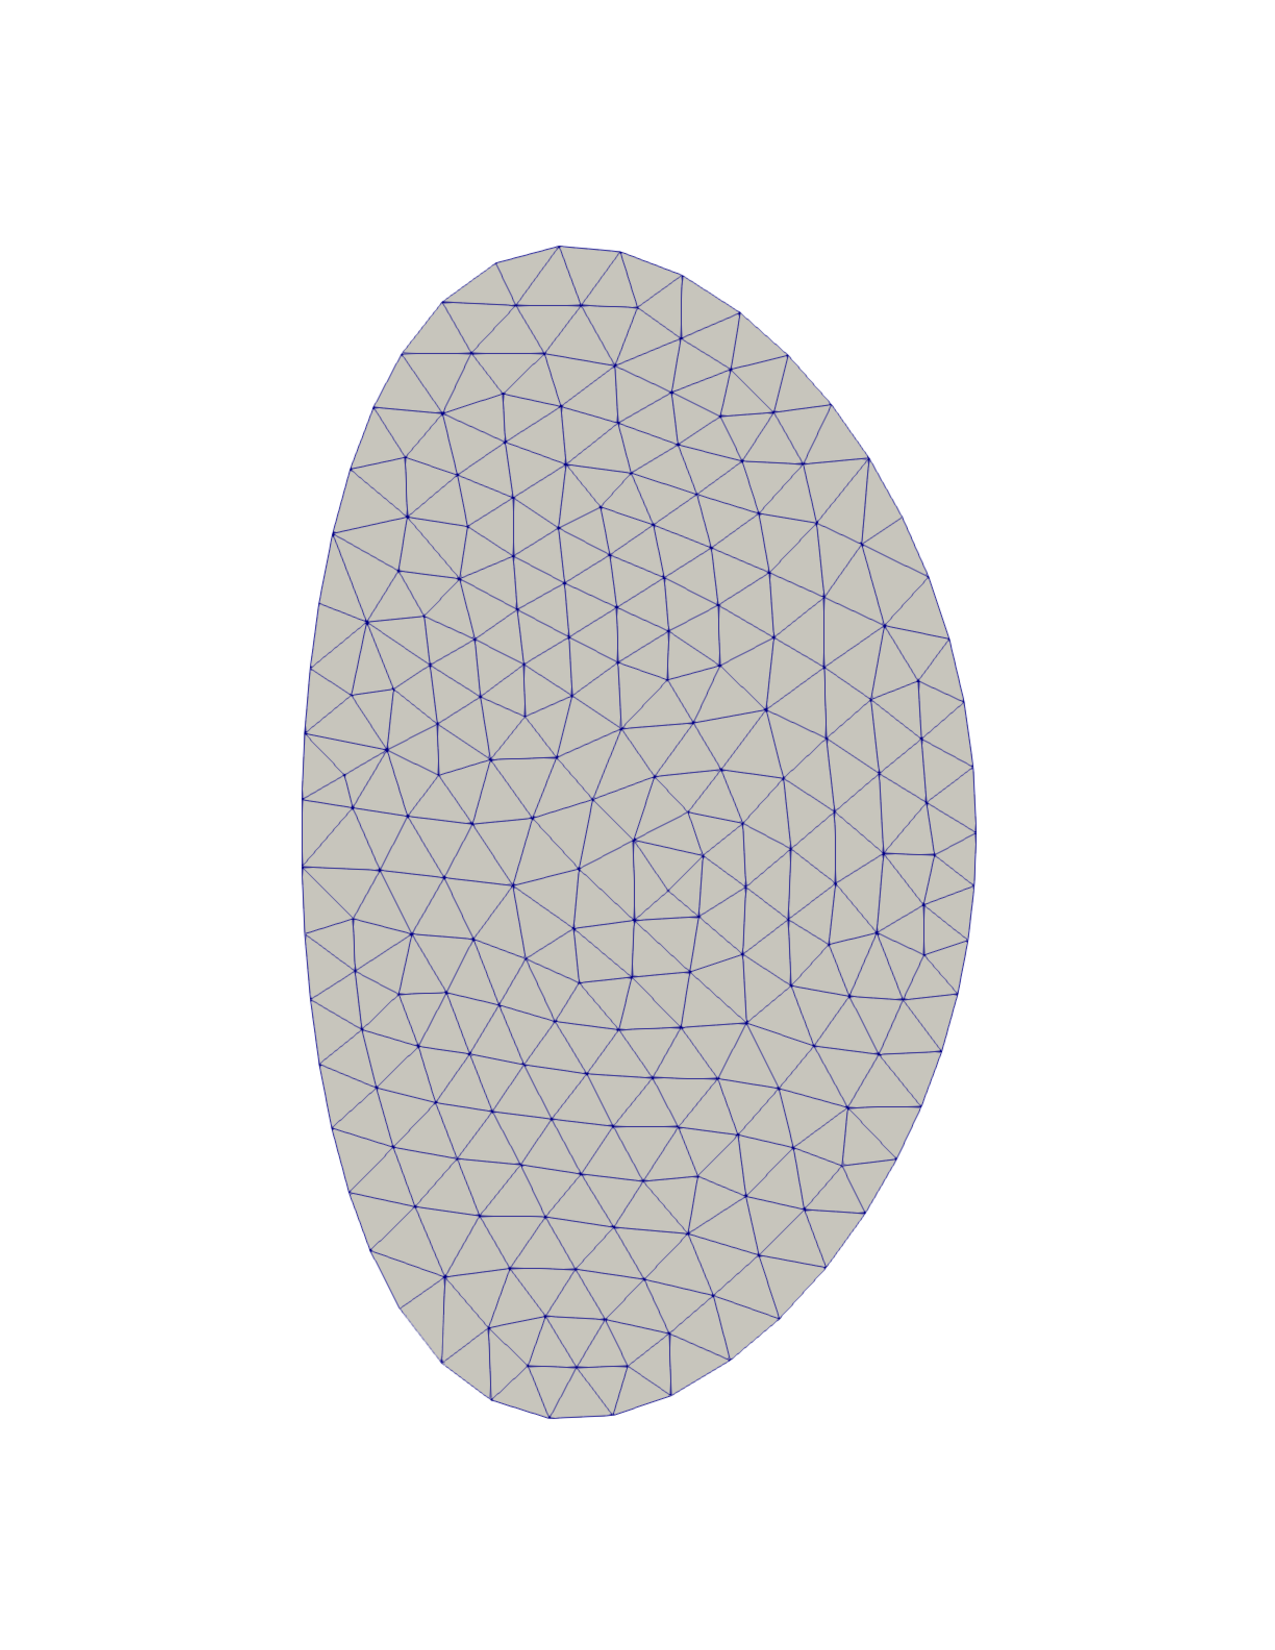
\includegraphics[width=3in]{./figures/meshgen-analytic-20pts-09.pdf}
\caption{Mesh with a parameterized vacuum region and different mesh size for model face (left) 0.2 (right) 0.09}
\label{fig:analytic-mesh}
\end{figure}

The figure~\ref{fig:analytic-mesh} presents the mesh generated by the input file above with two different mesh sizes.

%\begin{verbatim}
%numBdry 0
%numFace 1
%faceBdry 1 1
%outFile analytic-0.05
%meshSize 0.05
%useVacuumParams 1
%vacuumParams 1.65908 0.46 0.2 -0.02504 0.8
%numVacuumPts 50
%\end{verbatim}

%\begin{figure}
%\centering
%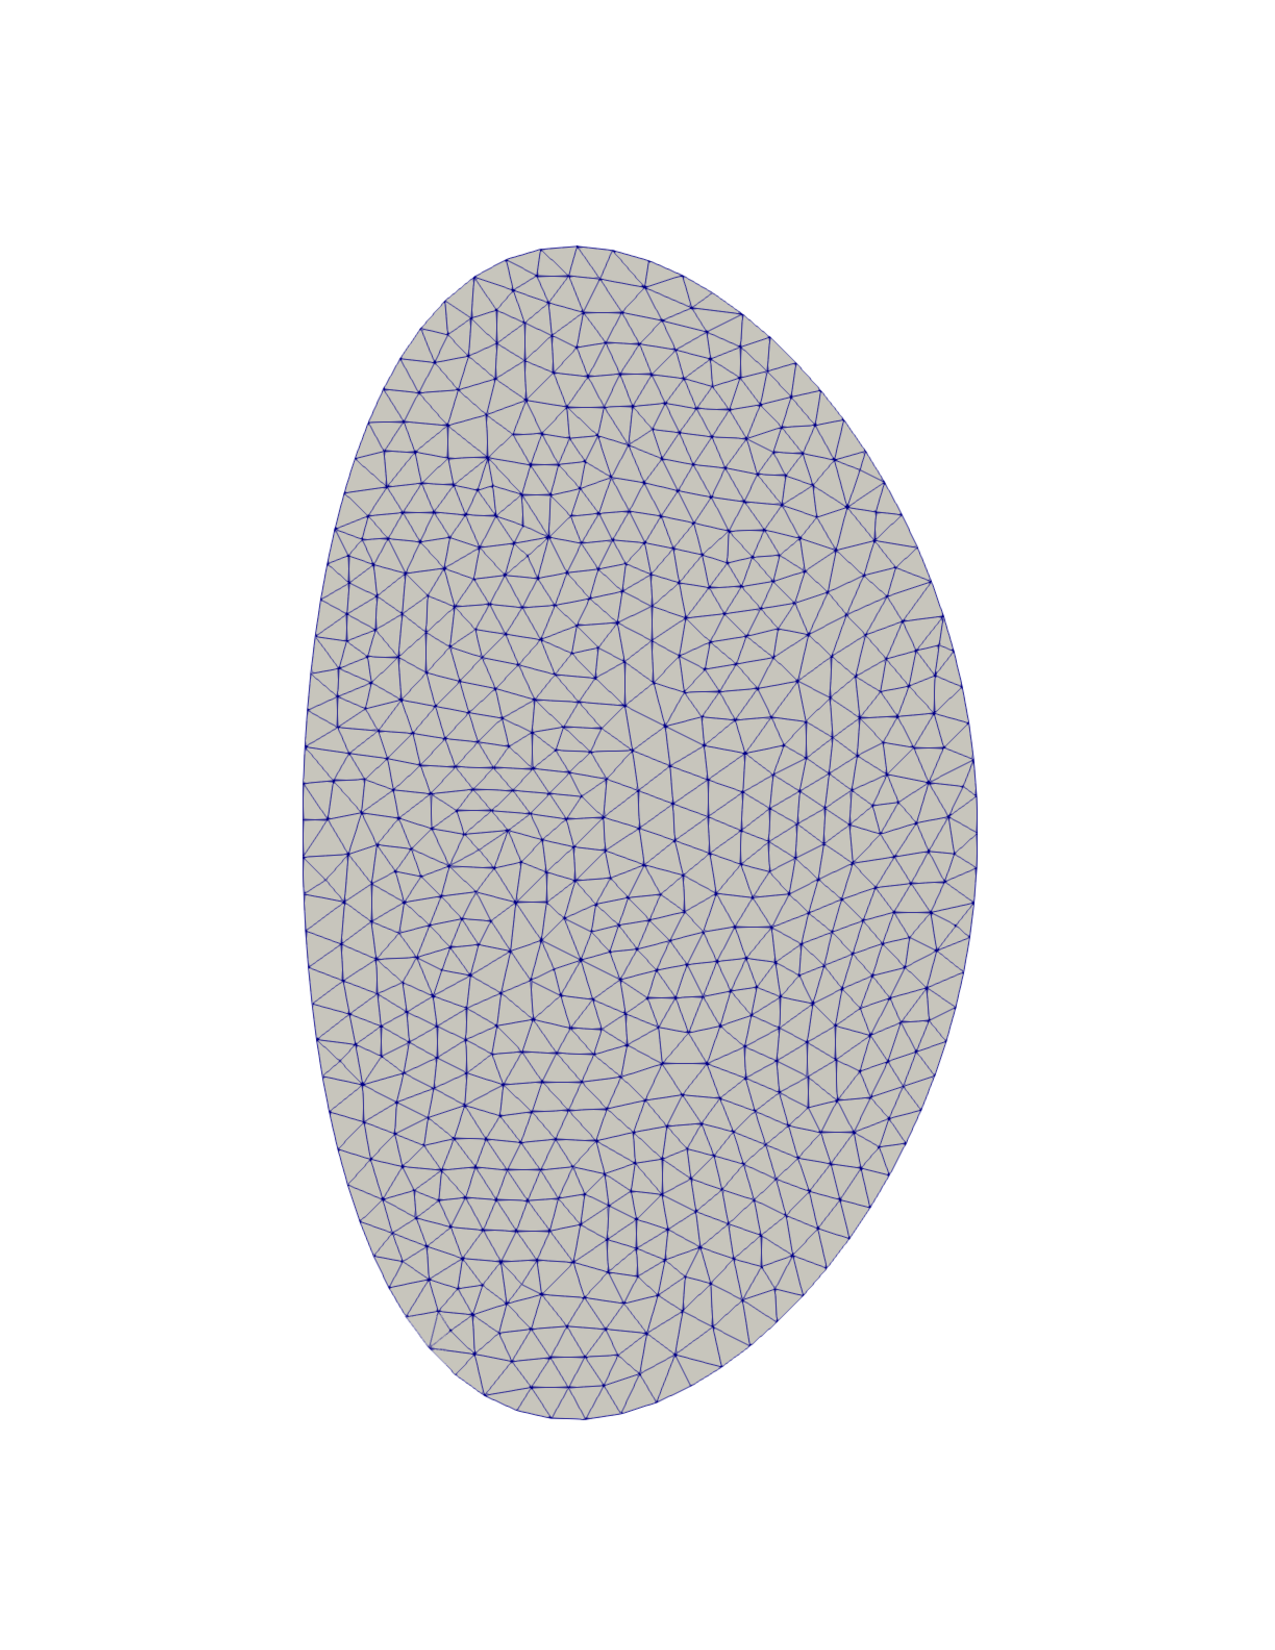
\includegraphics[width=3in]{./figures/meshgen-analytic-50pts-05.pdf}
%\caption[Mesh with parameterized vacuum region II]
%{A mesh with parameterized vacuum region of 50 interpolation points and mesh size 0.05}
%\label{fig:analytic-mesh-2}
%\end{figure}
%
%The figure~\ref{fig:analytic-mesh-2} presents the mesh generated by the input file above.

%%%%%%%%%%%%%%%%%%%%%%%%%%%%%%%%%%%%%%%%%
\subsubsection{Mesh with single boundary file}
%%%%%%%%%%%%%%%%%%%%%%%%%%%%%%%%%%%%%%%%%

\begin{verbatim}
numBdry 1
bdryFile loop1.dat 3 0.1
numFace 1
faceBdry 1 3 0.2
outFile input1
\end{verbatim}

\begin{figure}
\centering
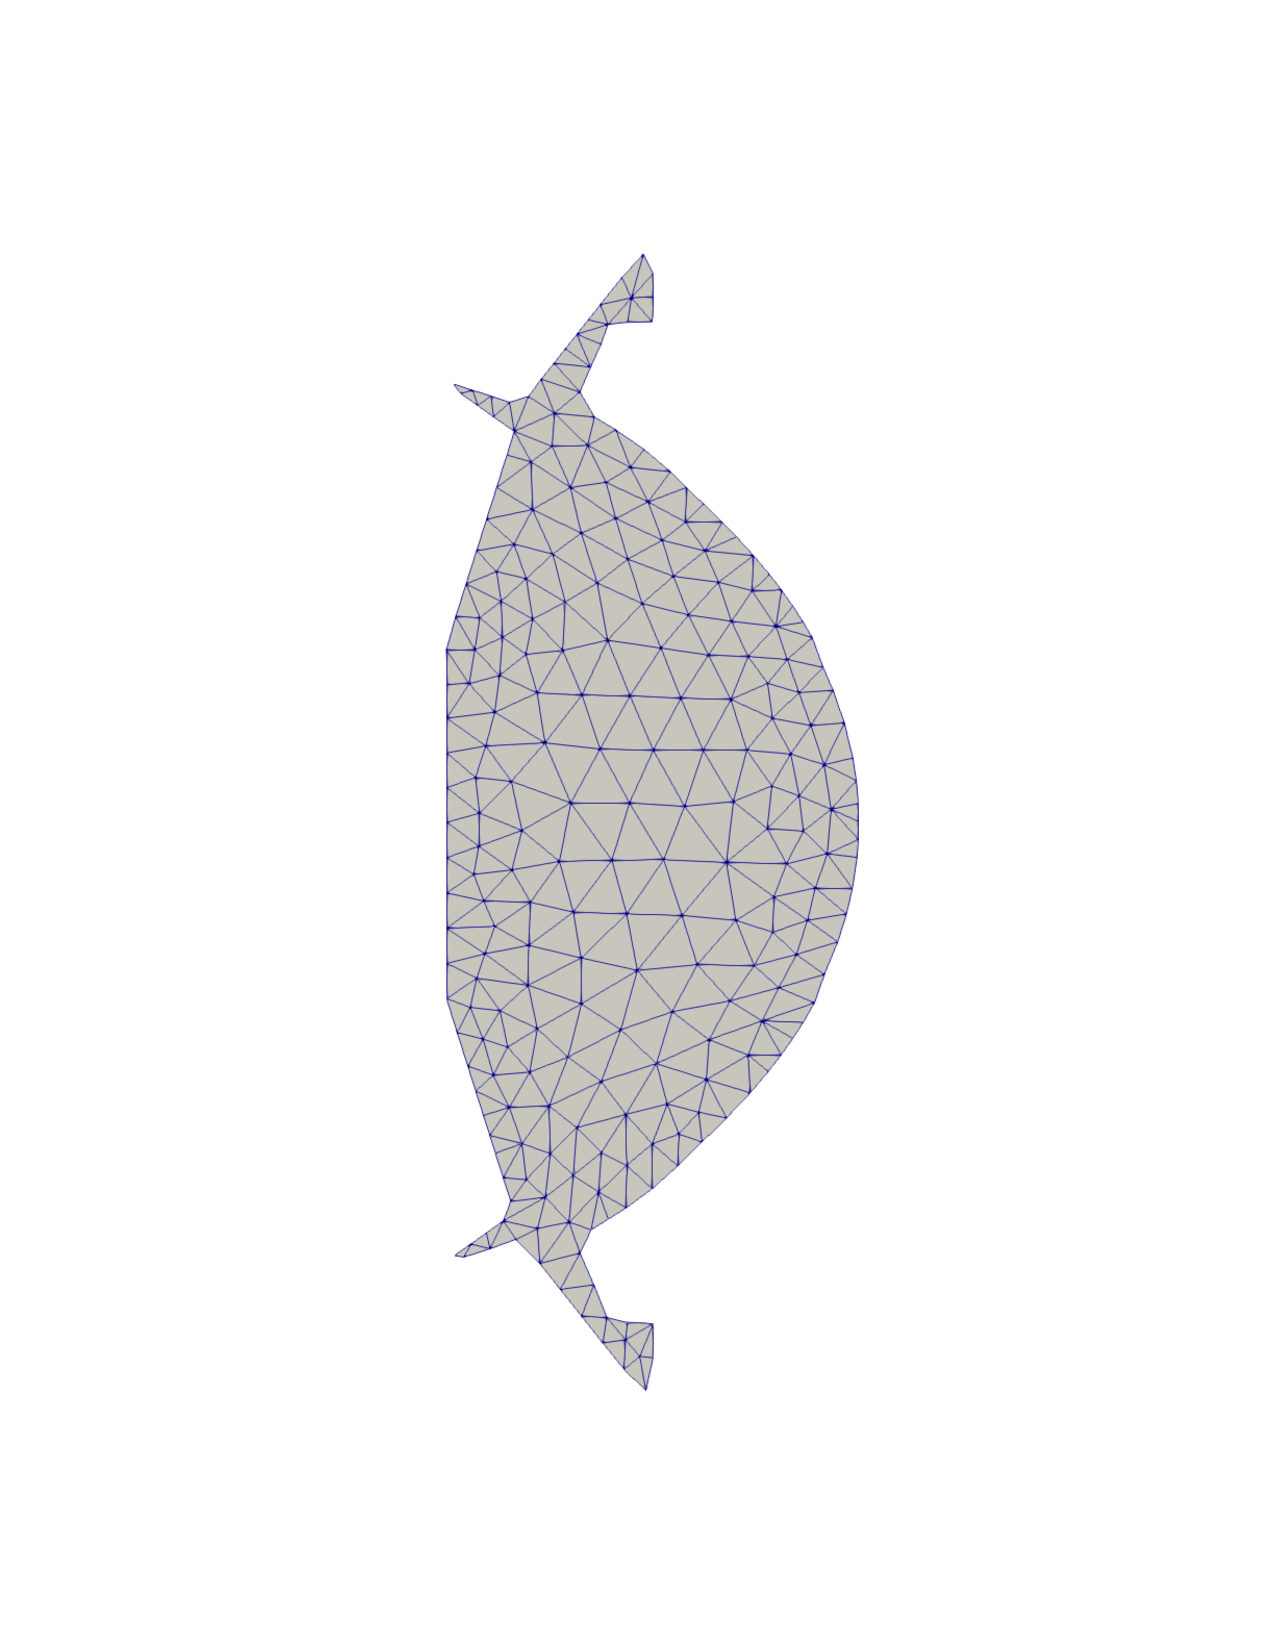
\includegraphics[width=3in]{./figures/meshgen-input1-novacuum.pdf}
\caption{Mesh with single boundary file and no vacuum wall}
\label{fig:input1}
\end{figure}

The figure~\ref{fig:input1} presents the mesh generated by the input file above.

%%%%%%%%%%%%%%%%%%%%%%%%%%%%%%%%%%%%%%%%%
%\subsubsection{Mesh with single boundary file and a vacuum wall} 
%%%%%%%%%%%%%%%%%%%%%%%%%%%%%%%%%%%%%%%%%
%\begin{verbatim}
%numBdry 1
%bdryFile loop1.dat 3 0.1
%
%thickWall 0 19 8 0.07
%useVacuum 2 9 0.01
%vacuumParams 1.8 1.5 0.4 0.0 2.5
%numVacuumPts 20
%
%numFace 1
%faceBdry  1 3 0.2
%outFile input1
%
%meshGradationRate 0.3
%\end{verbatim}
%
%\begin{figure}
%\centering
%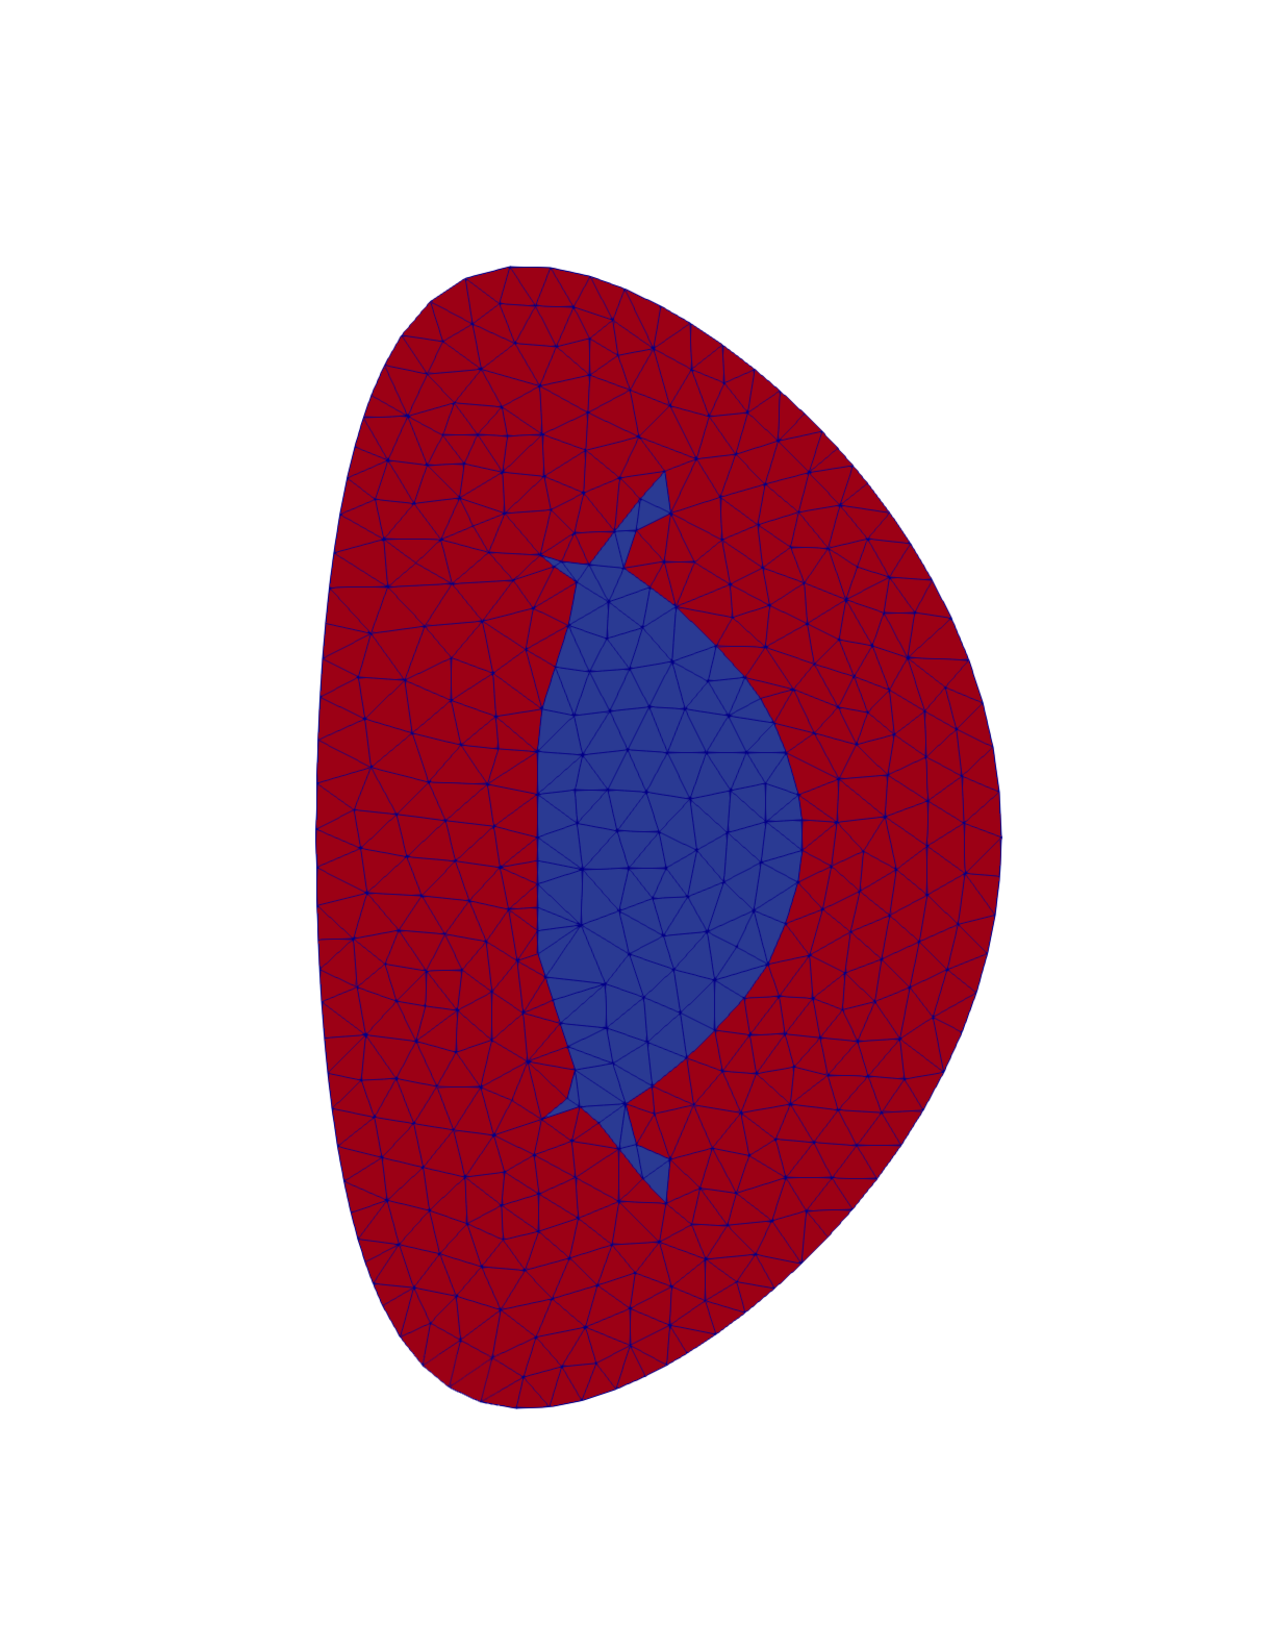
\includegraphics[width=3in]{./figures/meshgen-input1.pdf}
%\caption[Mesh with one boundary file and vacuum wall]
%{Mesh with one boundary file and vacuum wall}
%\label{fig:input1-vacuum}
%\end{figure}

%The figure~\ref{fig:input1-vacuum} presents the mesh generated by the input file above.

%%%%%%%%%%%%%%%%%%%%%%%%%%%%%%%%%%%%%%%%%
\subsubsection{Mesh with two boundary files and a parameterized vacuum wall}
%%%%%%%%%%%%%%%%%%%%%%%%%%%%%%%%%%%%%%%%%

This section presents a mesh created with two boundary files and a parameterized vacuum wall. This is equivalent to \texttt{Type 4} mesh of \texttt{m3dc1\_meshgen}.

\begin{verbatim}
numBdry 2
bddyFile loop1.pts 1 0.5
bdryFile loop2.pts 2 0.5
useVacuum 2 3 0.5
vacuumParams 8.25 8.0 0.2 0.0 12.5
numFace 3
faceBdry 1 1 0.7
faceBdry 2 1 2 0.5
faceBdry 2 2 3 0.7
meshGradationRate 1
outFile iter
\end{verbatim}

\begin{figure}
\centering
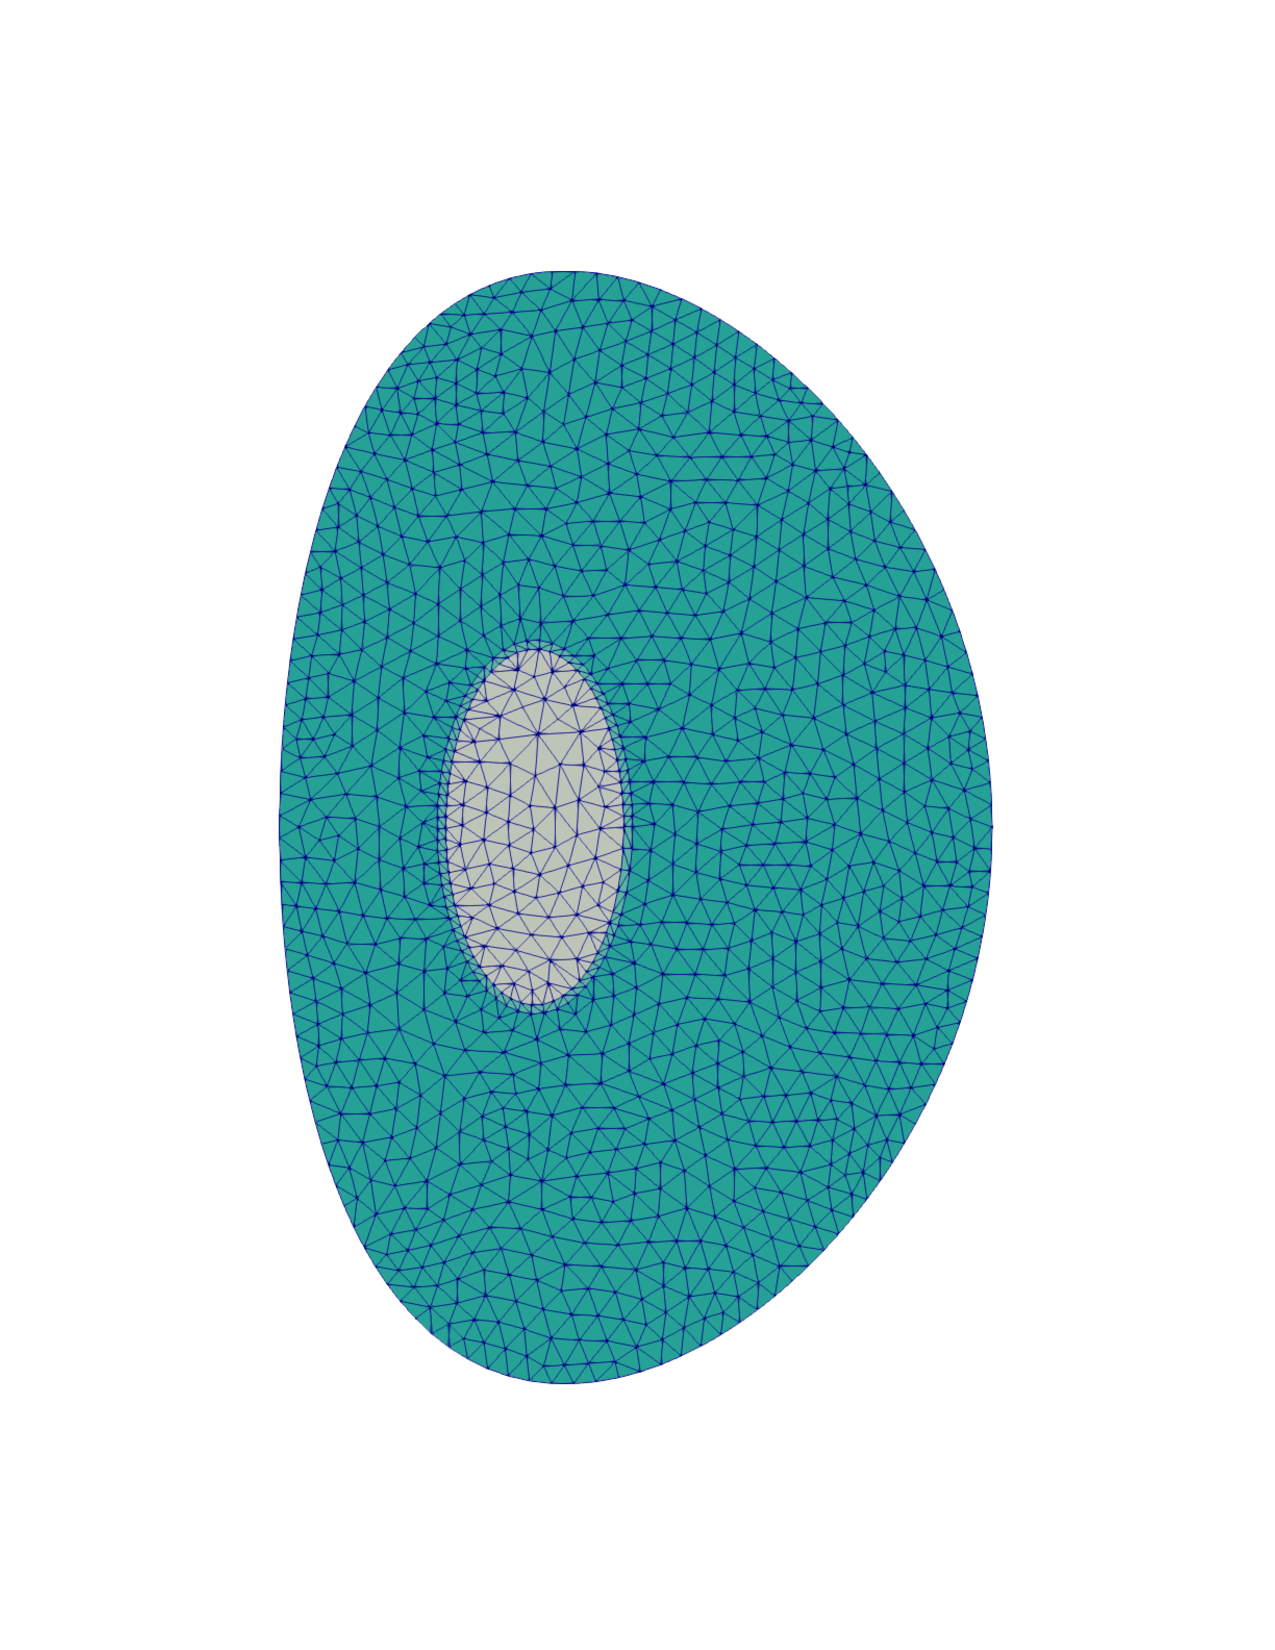
\includegraphics[width=3in]{./figures/meshgen-input2.pdf}
\caption{Mesh with two boundary files and a parameterized vacuum region}
\label{fig:input2}
\end{figure}

The figure~\ref{fig:input2} presents the mesh generated by the input file above. As you can see, the mesh in Figure ~\ref{fig:input2} and ~\ref{fig:meshgen-type4} are almost identical.


%%%%%%%%%%%%%%%%%%%%%%%%%%%%%%%%%%%%%%%%%
\subsubsection{Mesh with three boundary files}
%%%%%%%%%%%%%%%%%%%%%%%%%%%%%%%%%%%%%%%%%

\begin{figure}
\centering
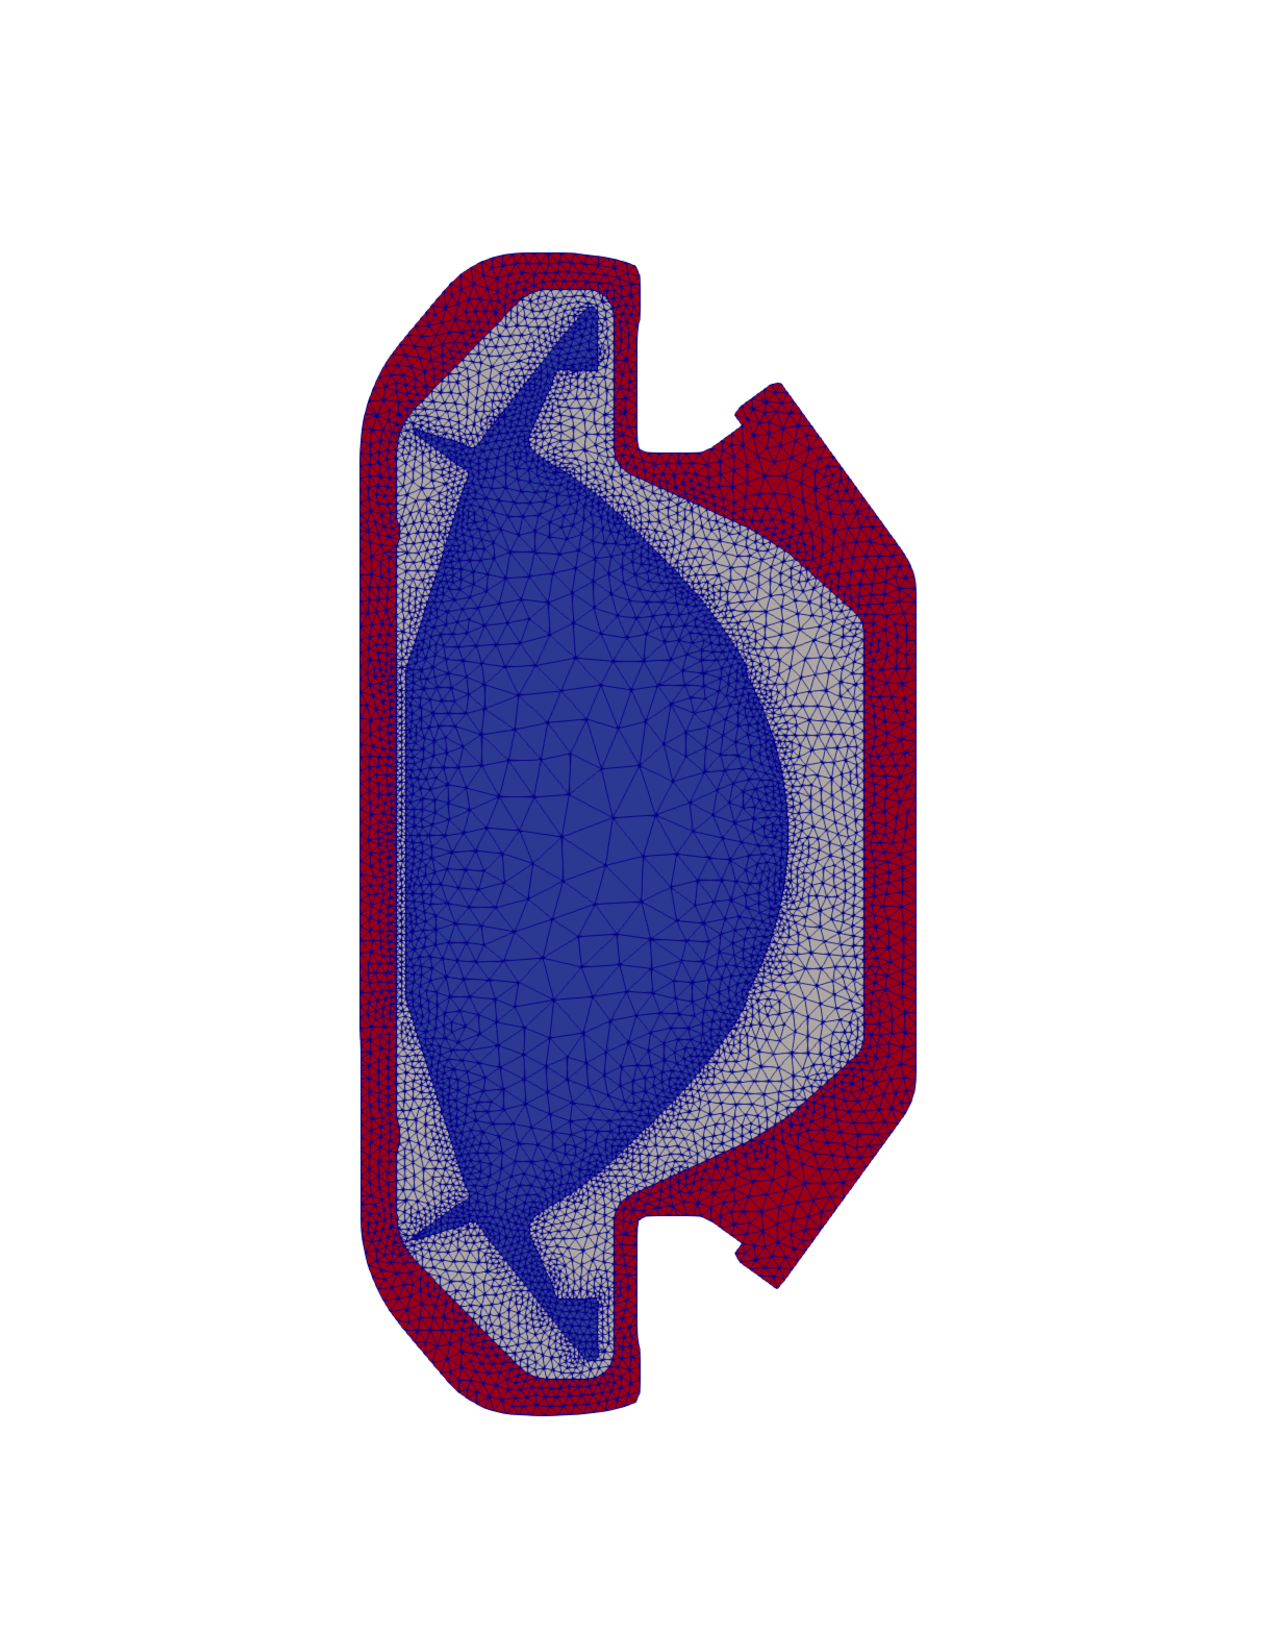
\includegraphics[width=3in]{./figures/meshgen-input3-novacuum.pdf}
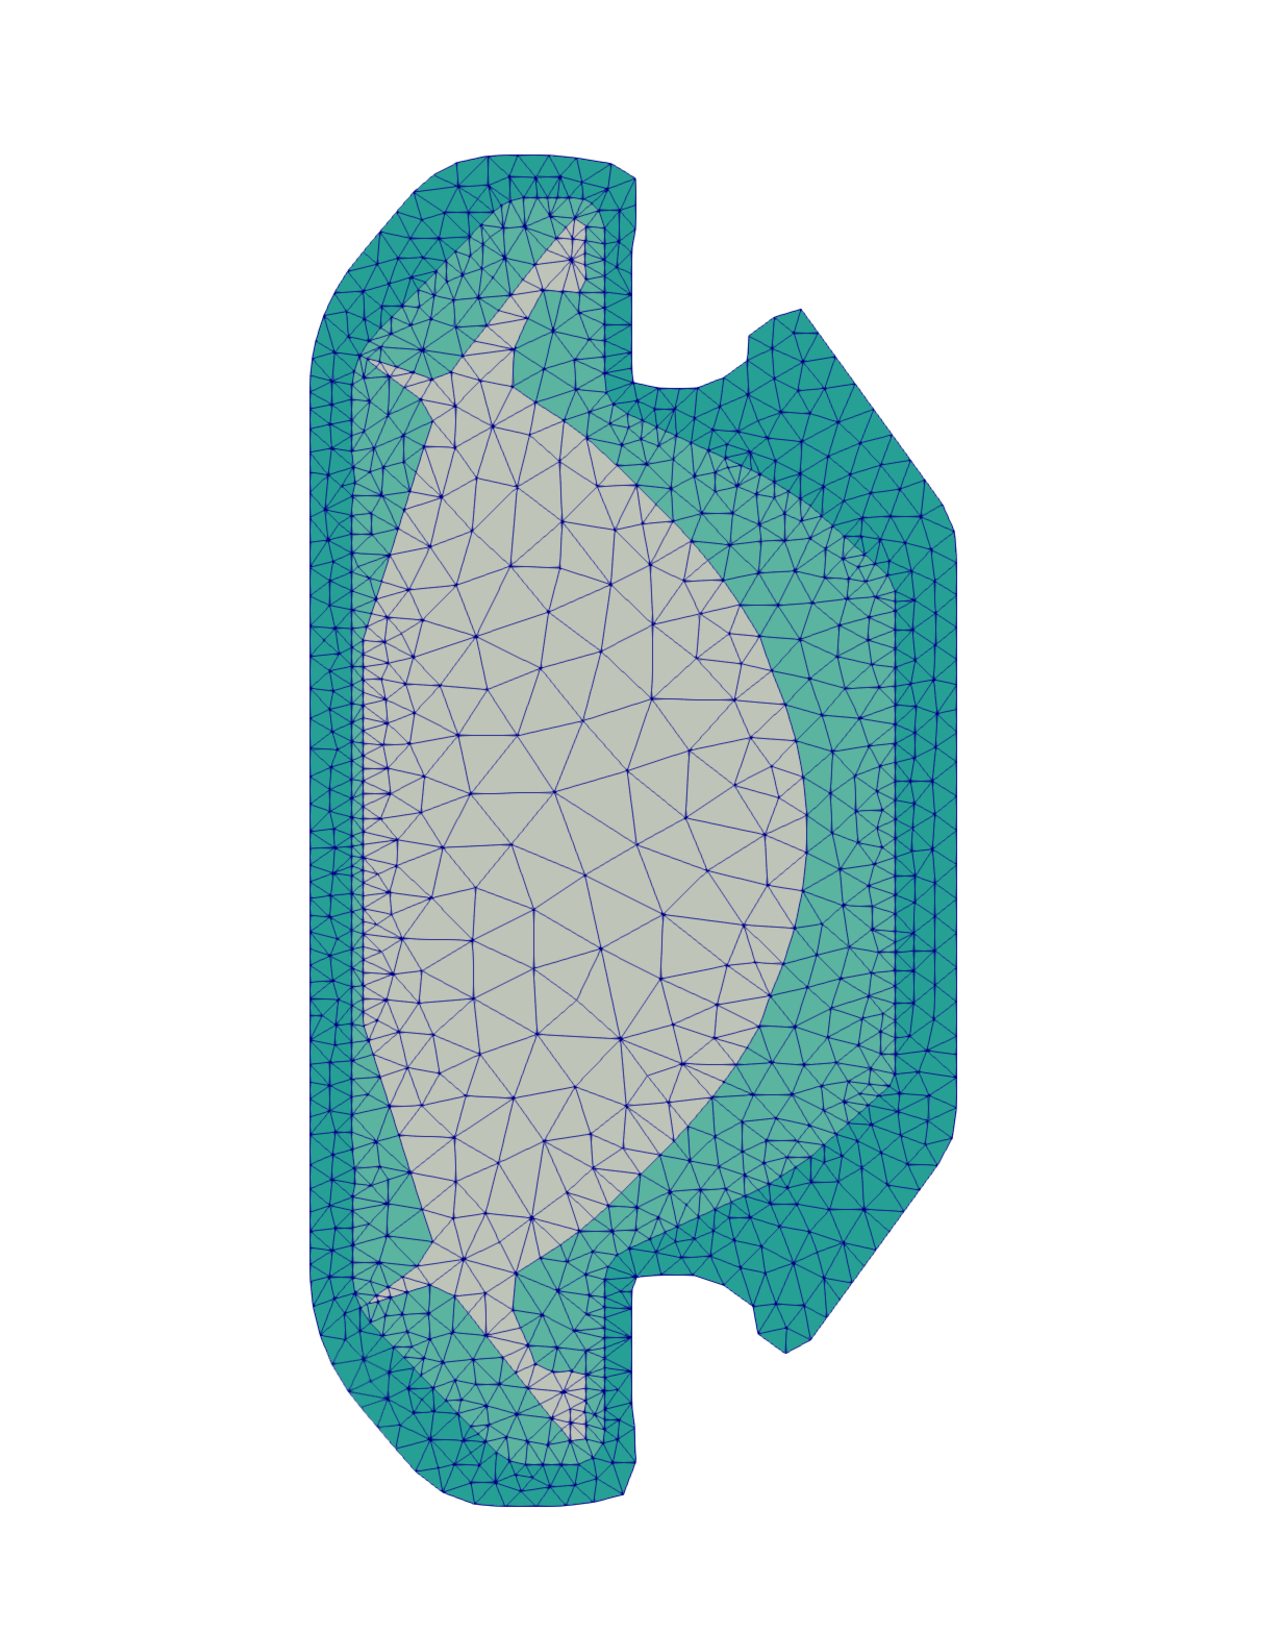
\includegraphics[width=3in]{./figures/meshgen-input3-novacuum2.pdf}
\caption
{Mesh with three boundary files and different meshGradationRate (left) 0.3 (right) 0.9}
\label{fig:input3-novacuum}
\end{figure}

\begin{verbatim}
numBdry 3
bdryFile loop1.dat 3 0.1
bdryFile loop2.dat 10 0.05
bdryFile loop3.dat 11 0.09

numFace 3
faceBdry  1 3 0.2
faceBdry  2 3 10 0.1
faceBdry  2 10 11 0.09

outFile input3
\end{verbatim}

The figure~\ref{fig:input3-novacuum} presents the mesh generated by the input file above.

%%%%%%%%%%%%%%%%%%%%%%%%%%%%%%%%%%%%%%%%%
\subsubsection{Mesh with seven boundary files and a vacuum wall}
%%%%%%%%%%%%%%%%%%%%%%%%%%%%%%%%%%%%%%%%%

\begin{figure}
\centering
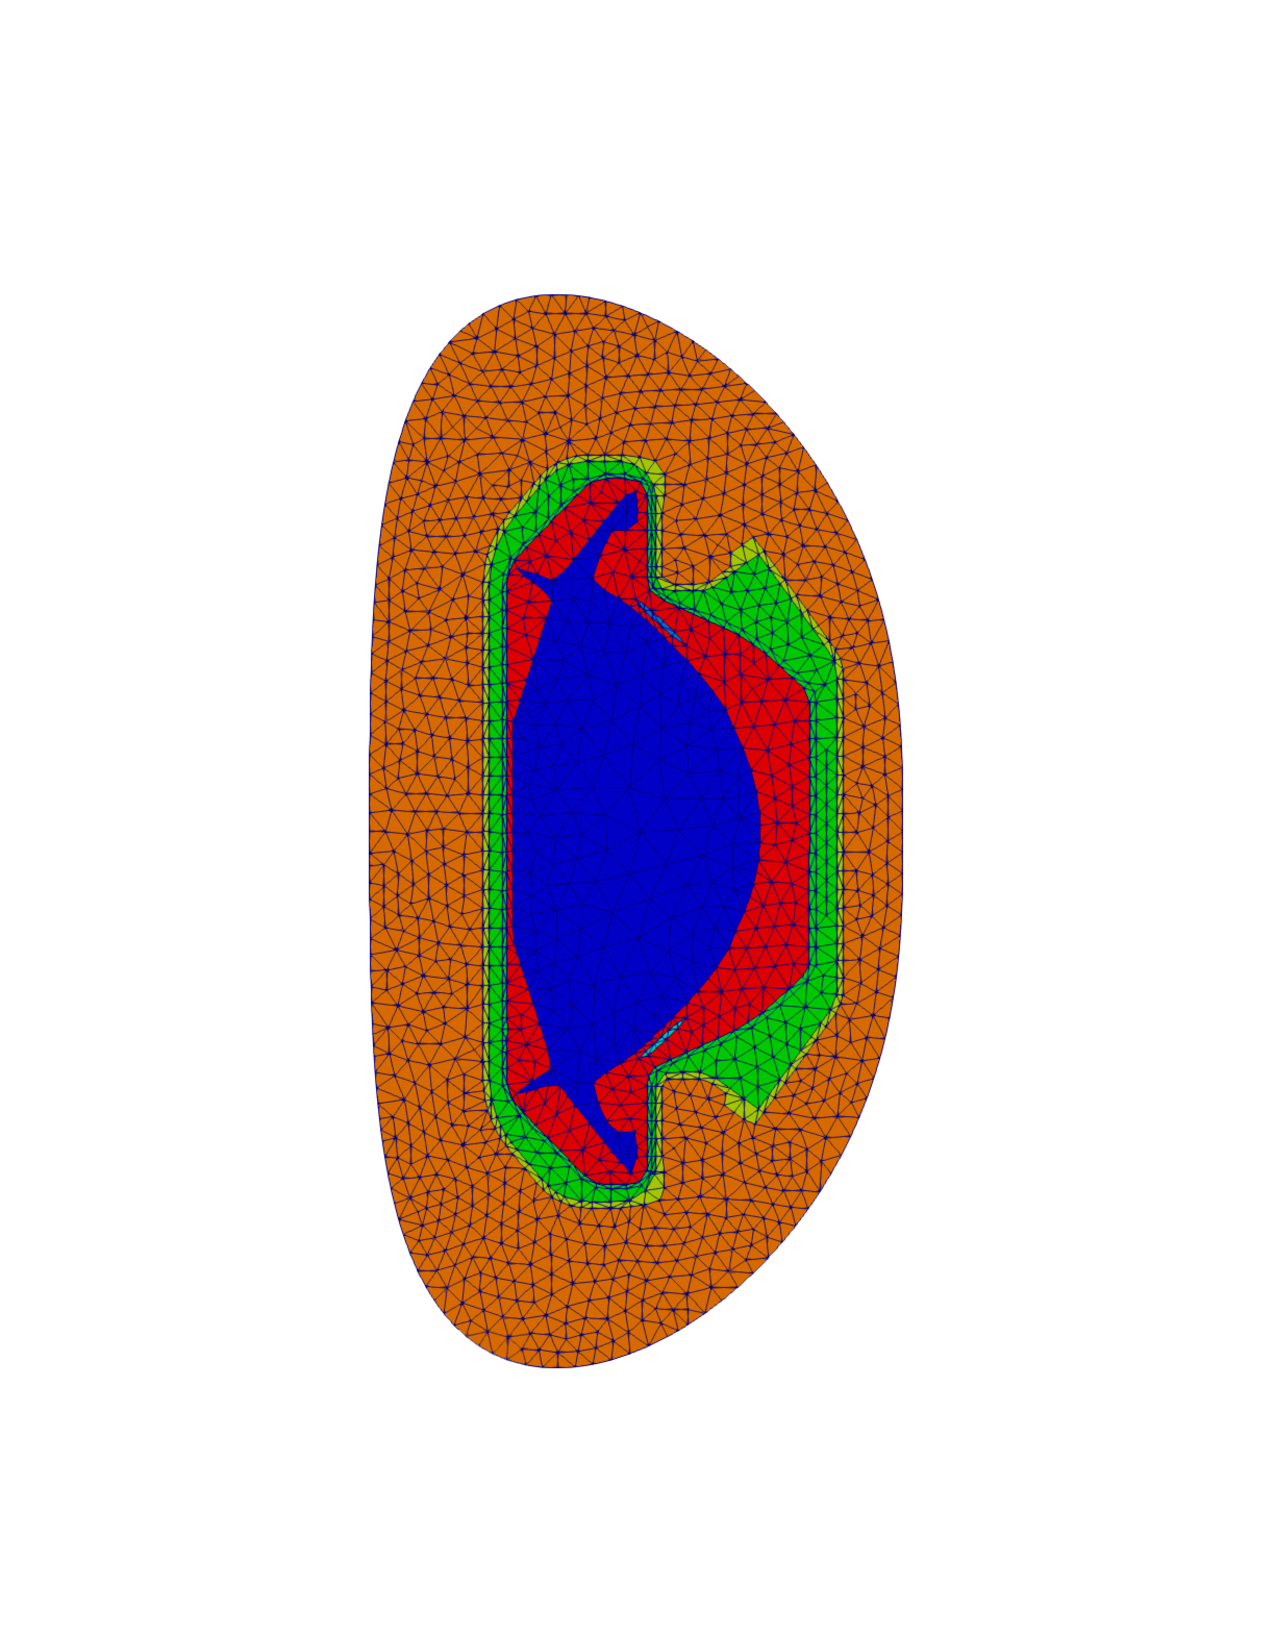
\includegraphics[width=4in]{./figures/meshgen-input7.pdf}
\caption{Mesh with seven boundary files and a parameterized vacuum wall}
\label{fig:input7-vacuum}
\end{figure}

\begin{verbatim}
numBdry 7
bdryFile loop1.dat 3 0.2
bdryFile loop2.dat 10 0.3
bdryFile loop3.dat 11 0.4
bdryFile loop4.dat 21 0.4
bdryFile loop5.dat 25 0.4
bdryFile loop6.dat 17 0.2
bdryFile loop7.dat 19 0.1

useVacuum 1 9 0.1
vacuumParams 1.8 1.5 0.4 0.0 2.5

numFace 8
faceBdry  1 3 0.2
faceBdry  1 10 0.3
faceBdry  1 11 0.1
faceBdry  2 21 25 0.2
faceBdry  2 25 17 0.09
faceBdry  2 17 19 0.1
faceBdry  2 19 9 0.1
faceBdry  4 3 10 11 21 0.11

outFile input7
\end{verbatim}

The figure~\ref{fig:input7-vacuum} presents the mesh generated by the input file above.

%%%%%%%%%%%%%%%%%%%%%%%%%%%%%%%%%%%%%%%%%
\subsubsection{Mesh with finite thickness wall and layers}
%%%%%%%%%%%%%%%%%%%%%%%%%%%%%%%%%%%%%%%%%

\begin{figure}
\centering
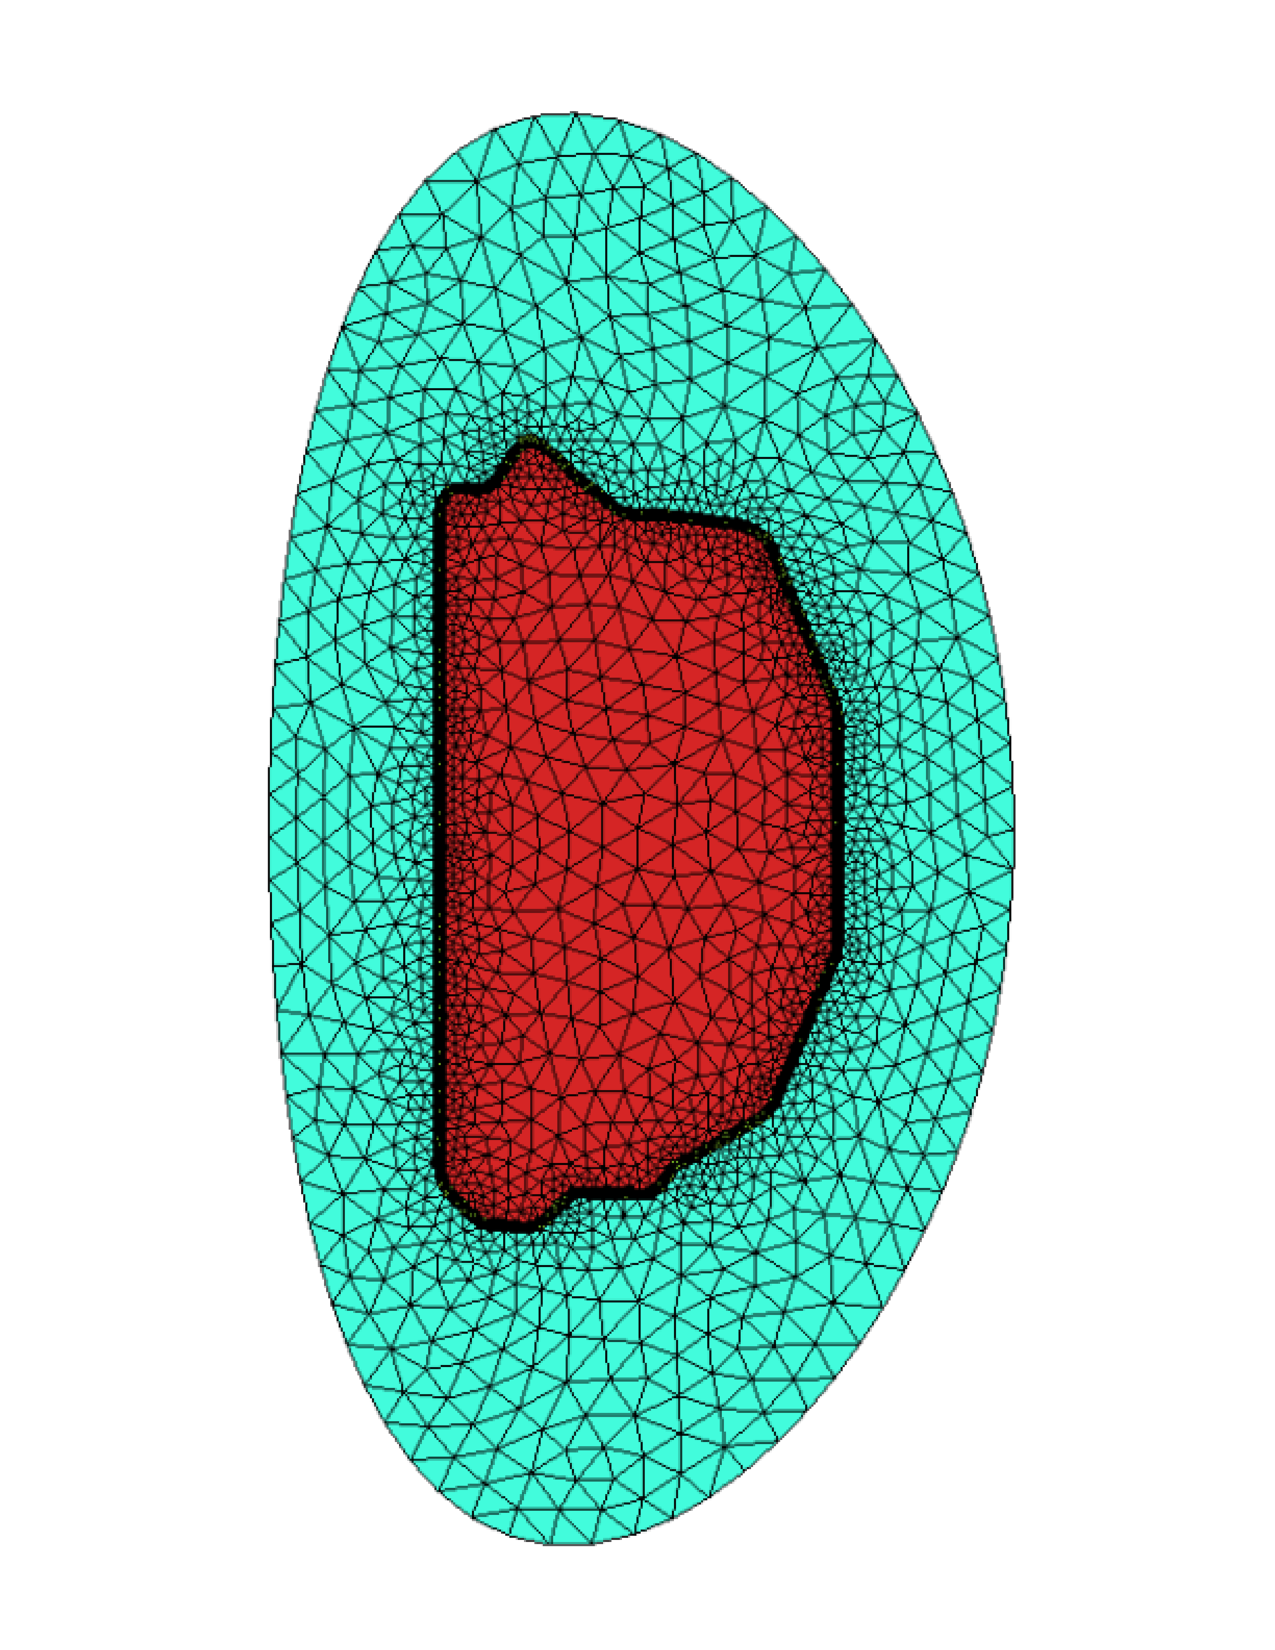
\includegraphics[width=3.5in]{./figures/FiniteThicknessWall-full.pdf}
\caption
{Add Caption Here}
\label{fig:thickness-full}
\end{figure}

\begin{figure}
\centering
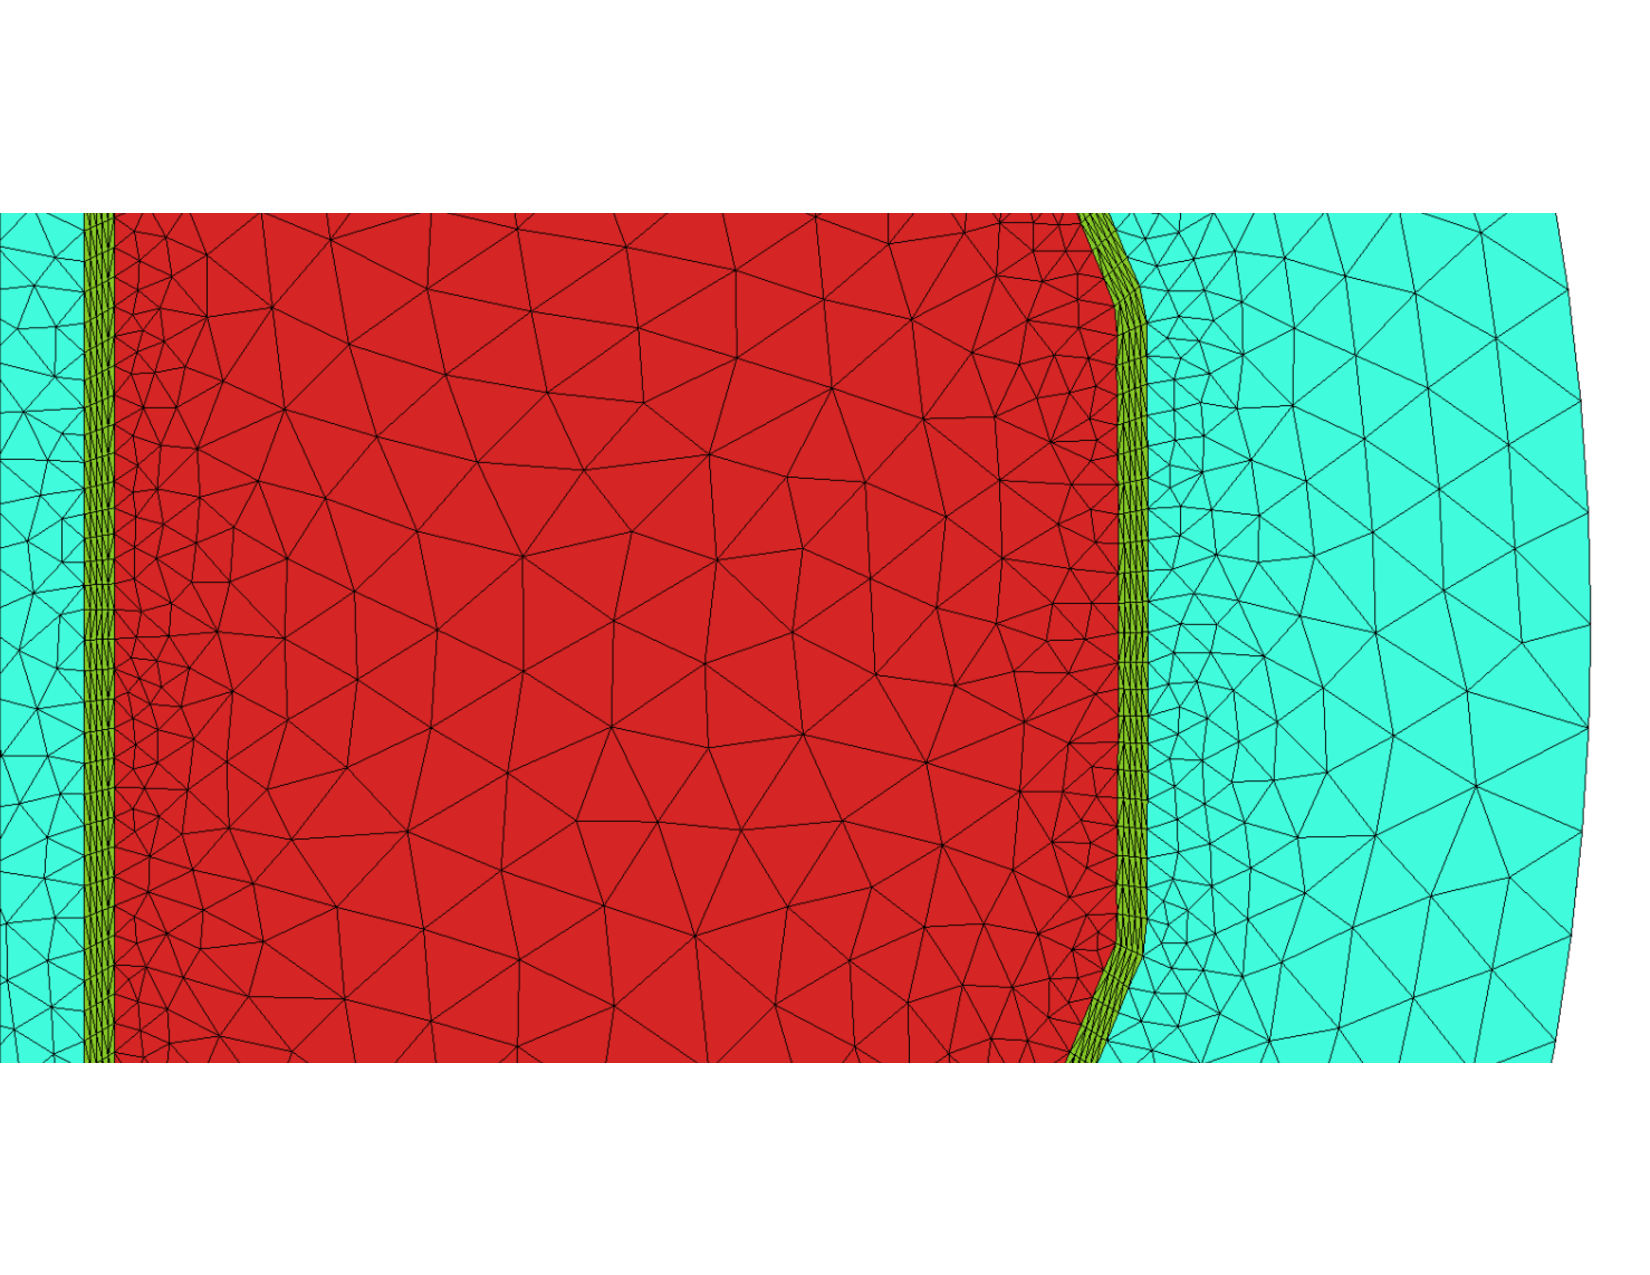
\includegraphics[width=2.5in]{./figures/FiniteThicknessWall-zoom1.pdf}
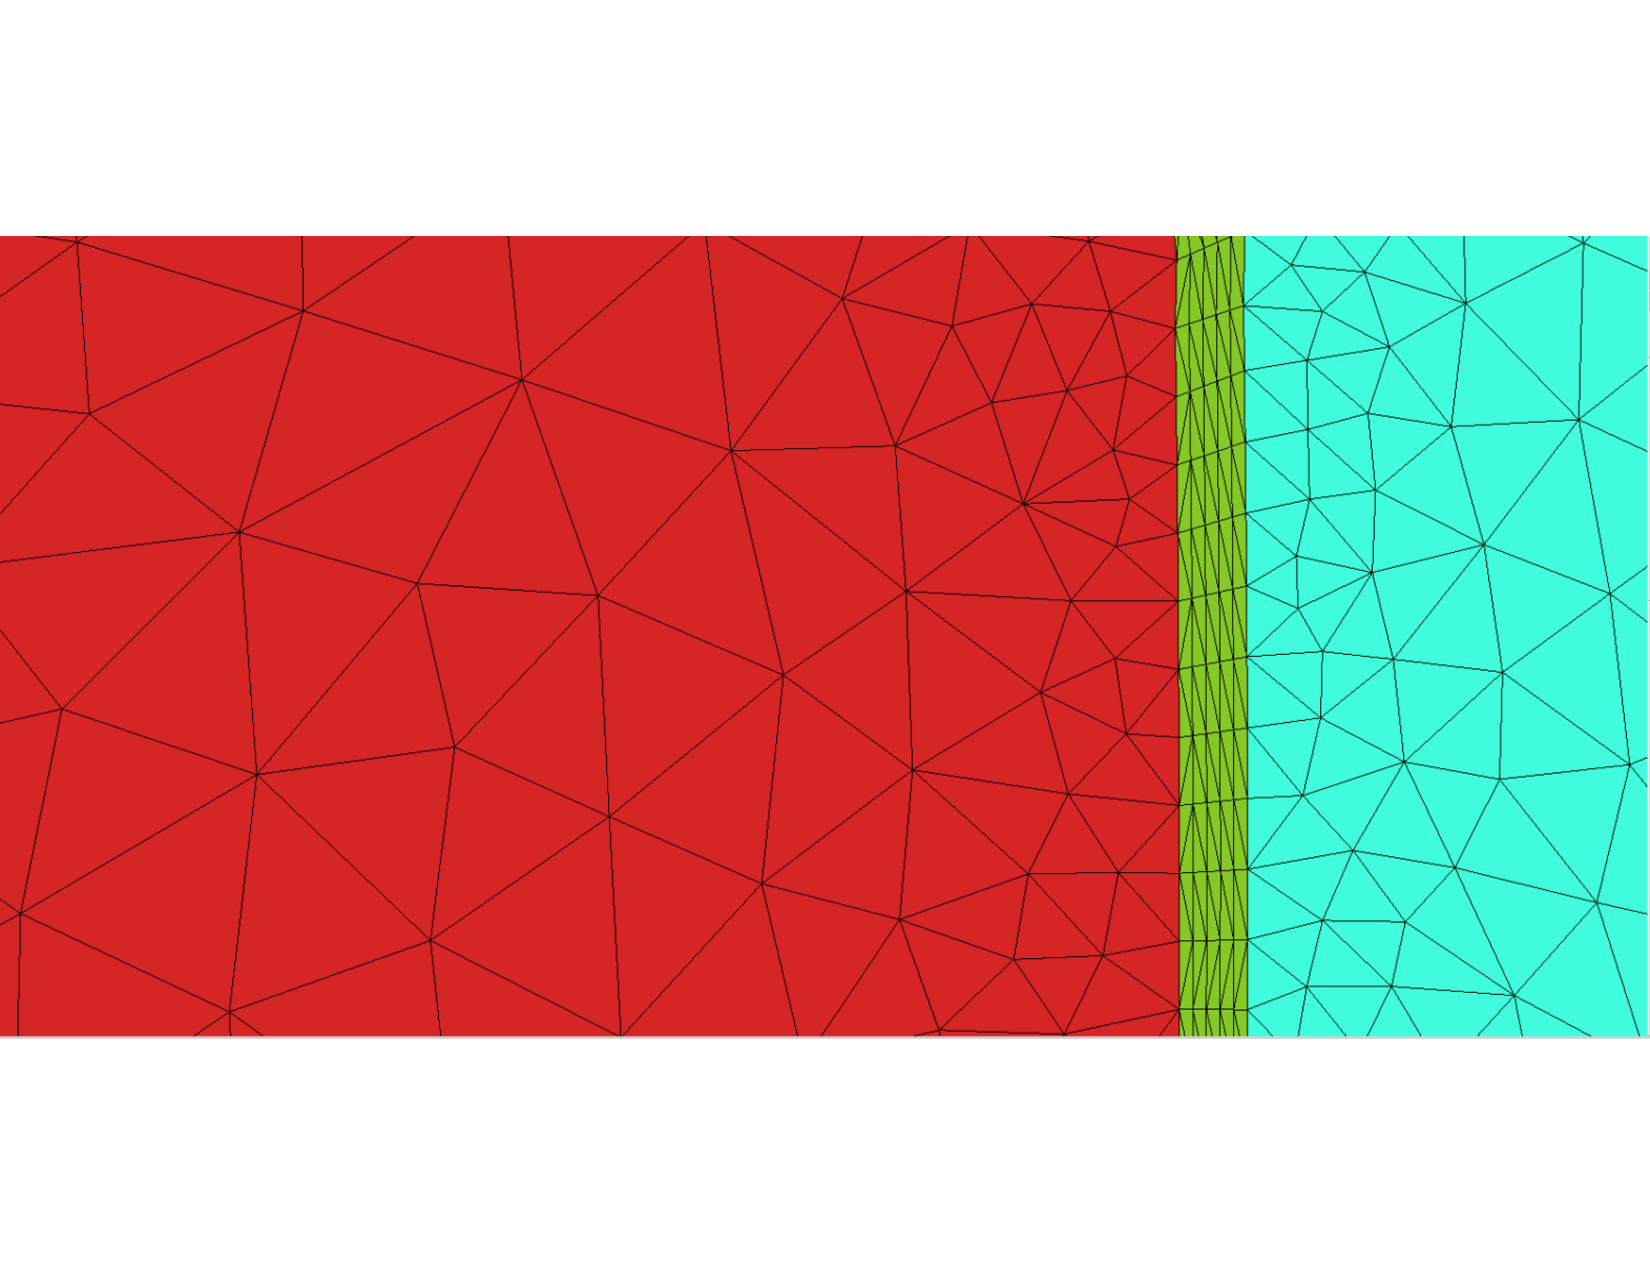
\includegraphics[width=2.5in]{./figures/FiniteThicknessWall-zoom2.pdf}
\caption
{Add Caption Here}
\label{fig:thickness-zoom}
\end{figure}

Add text here

%%%%%%%%%%%%%%%%%%%%%%%%%%%%%%%%%%%%%%%%%
\subsection{polar\_meshgen}
\label{ch:polar-gen}
%%%%%%%%%%%%%%%%%%%%%%%%%%%%%%%%%%%%%%%%%
\texttt{polar\_meshgen} requires an ascii file of arbitrary name that contains input parameters as the following:
\begin{itemize}
\item inFile: input file name containing equilibrium generation by jsolver
\item outFile: output file name to save model and mesh
\item meshSize: relative mesh size for each region (default 0.05)
\item reorder: if 1, reorder PUMI mesh based on adjacency (default: 0) and generate vtk folders for mesh visualization. The mesh before and after reodering is saved in \texttt{original-mesh.vtk} and \texttt{reordered-mesh.vtk}, respectively. Note that the element order of Simmetrix mesh is not affected.
\end{itemize}

The following presents an example input file ``\texttt{polar\_input}''.
\begin{verbatim}
inFile POLAR
outFile polar
meshSize 0.04
\end{verbatim}

To run \texttt{polar\_meshgen}, place \texttt{polar\_input} and \texttt{POLAR} in your work folder and do ``\texttt{polar\_meshgen polar\_input}''. The program will read \texttt{POLAR} and generate various model and mesh files starting with ``polar''. For instance, \texttt{polar-2K0.smb, pol-2K.sms, pol-2K.vtk, polar.dmg, polar.smd, polar.txt}. If the resulting mesh is too fine, increase the value of \texttt{meshSize}. If the resulting mesh is too coarse, decrease the value of \texttt{meshSize}. If \texttt{meshSize} is not specified in the input file, the default value is 0.05.   

The program \texttt{read\_jsolver} generates equilibrium and stores in the file \texttt{POLAR}. Given the input file \texttt{POLAR}, \texttt{m3dc1\_meshgen} generates the following files:
\begin{itemize}
\item	model.dmg: PUMI-readable model file
\item	model.txt: M3DC1-readable model file
\item	mesh0.smb: PUMI/M3DC1-readable mesh file
\item	mesh.vtk: Paraview data files
\item	norm\_curv: ascii file containing nodes' normal/curvature information
\end{itemize} 

%%%%%%%%%%%%%%%%%%%%%%%%%%%%%%%%%%%%%%%%%
\subsection{Mesh Control with SimModeler}
SimModeler is a graphical user interface to the Simmetrix geometry and mesh generation software. In cases where the currently available capabilities of m3dc1\_meshgen do not provide a satisfactory mesh, SimModeler can be used to apply alternative mesh control information to the Tokamak cross section geometry to generate different meshes. The information below indicates the application of a subset of the mesh controls that can be applied. For additional information of the full range of SimModeler mesh control options see: ********** FILL IN POINTER TO SIMMETRIX DOCUMENTATION *****
\label{ch:simmodeler}
%%%%%%%%%%%%%%%%%%%%%%%%%%%%%%%%%%%%%%%%%
(Contributed by D. Pfefferle on 4/27/16) On PPPL Portal, load a module \texttt{simmodeler} and run it.
\begin{enumerate}
\item From the menu \texttt{"File$\rightarrow$Open Model"}, load a model file (\texttt{.smd}) generated by \texttt{m3dc1\_meshgen}
\item In the upper panel, in the views section, click on \texttt{Front} to view the model, then go to \texttt{Meshing} tab
\item Select outer region, click \texttt{+} in \texttt{Mesh Attributes} and select \texttt{Mesh Size$\rightarrow$relative}. 
Enter a value (typically 0.1)
\item Select wall region, click \texttt{+} in \texttt{Mesh Attributes} and select \texttt{Mesh Size$\rightarrow$relative}. 
Enter a value (typically 0.02)
\item Select inner region, click \texttt{+} in \texttt{Mesh Attributes} and select \texttt{Mesh Size$\rightarrow$relative}. 
Enter a value (typically 0.04). Here, one can already generate the mesh by clicking on \texttt{Generate Mesh} and verify if the mesh sizes are suitable 
\item 	Select both inner and wall regions (holding shift key), click \texttt{+} in \texttt{Mesh Attributes} and select \texttt{Mesh Size$\rightarrow$relative}. Enter a function, e.g. \texttt{0.01$\times$abs(\$y+1.5)\^{}2+0.004} to specify an anisotropic mesh density on top of previous settings
\\ There are many available parameters for fine-tuning the mesh density.  For example, \texttt{Mesh Curvature Refinement} with parameter packs more elements near the edges of the resistive wall. 
\item \texttt{Generate Mesh} and \texttt{Show Mesh} to view result in new windows
\item If the result is satisfactory, from the menu \texttt{File$\rightarrow$Save Mesh}, give it a meaningful name with the extension \texttt{.sms}. The original model file \texttt{.smd} has been automatically saved by the program with your mesh modifications.
\item Close \texttt{simmodeler} then it will release a license. Until you quit Simmodeler, no one cannot run neither \texttt{m3dc1\_meshgen} nor \texttt{simmodeler}.
\item Copy the \texttt{.txt, .smd} and \texttt{.sms} files to the simulation directory and run the following splitting routine to obtain PUMI-readable \texttt{.smb} mesh files.
\newline\newline
\texttt{/p/tsc/C1/m3dc1-sunfire.r6-1.5/bin/part\_mesh.sh model\_file.smd mesh\_file.sms X}, 
where \texttt{X} is the number of parts you need in the \texttt{.smb} mesh.
\item Modify the \texttt{C1input} file accordingly
\newline\newline
\texttt{mesh\_filename = `part.smb'
\\
mesh\_model = `filename.txt'
}
\end{enumerate}

%%%%%%%%%%%%%%%%%%%%%%%%%%%%%%%%%%%%%%%%%
\subsection{Mesh Partitioning}
\label{ch:mesh-ptn}
%%%%%%%%%%%%%%%%%%%%%%%%%%%%%%%%%%%%%%%%%

\subsubsection{Splitting}

The program \texttt{split\_smb} increases the number of parts in a mesh from \texttt{P} to \texttt{N} (\texttt{P$<$N}). 
In each machine, the program \texttt{split\_smb} is availble in \texttt{\$SCOREC\_UTIL\_DIR} provided in \texttt{hostname.mk} file.

In order to split \texttt{P}-part mesh to \texttt{N} parts (\texttt{N$>$P}), run
\texttt{"mpirun -np N ./split\_smb input-mesh(.smb) output-mesh(.smb) X"}
\begin{itemize}
\item	the file extension of input-mesh should be .smb 
\item	the file extension of output-mesh should be .smb
\item	\texttt{N} is the number of parts in the output mesh
\item	For a \texttt{P}-part input mesh, \texttt{X} must be \texttt{N/P}
\item	For both input and output mesh, do not specify a number before the file extension
\item	\texttt{split\_smb} will insert a number in the output mesh file. The number represents a global part ID.
\item	Make sure that the output mesh doesn't have any empty part. Otherwise, the program crashes with the following error message:
\newline
\texttt{APF warning: 1 empty parts}
\newline
\texttt{split\_smb: \ldots/mds/mds.c:614: check\_ent: Assertion `e $>$= 0' failed}
\end{itemize}

Examples on portal:
\begin{enumerate}
\item To split a serial (1-part) mesh to 6 parts, run\\
 \texttt{"mpirun -np 6 ./split\_smb struct-curveDomain.smb part.smb 6"}
\begin{itemize}
\item	Input mesh: struct-curveDomain0.smb 
\item	Output mesh: part0.smb, part1.smb, part2.smb, part3.smb, part4.smb, part5.smb
\end{itemize}

\item To split a 2-part mesh to 6 parts, run
 \texttt{"mpirun -np 6 ./split\_smb  struct-curveDomain.smb part.smb 3"}
\begin{itemize}
\item	Input mesh: struct-curveDomain0.smb, struct-curveDomain1.smb
\item	Output mesh: part0.smb, part1.smb, part2.smb, part3.smb, part4.smb, part5.smb
\end{itemize}
\end{enumerate}

See \texttt{readme.split\_smb} for detailed instructions and trouble shooting tips.

%%%%%%%%%%%%%%%%%%%%%%%%%%%%%%%%%%%%%%%%%
\subsubsection{Mesh Merging}
\label{ch:mesh-mg}
%%%%%%%%%%%%%%%%%%%%%%%%%%%%%%%%%%%%%%%%%

The program \texttt{collapse} decreases the number of parts in a mesh from \texttt{N} to \texttt{P} (\texttt{P$<$N}). 
In each machine, the program \texttt{collapse} is availble in \texttt{\$SCOREC\_UTIL\_DIR} provided in \texttt{hostname.mk} file.

In order to merge \texttt{N}-part .smb mesh to \texttt{P} parts (\texttt{P$>$0}), run
\texttt{"mpirun -np N ./collapse input-mesh(.smb) output-mesh(.smb) X"}
\begin{itemize}
\item	the file extension of input-mesh should be .smb 
\item	the file extension of output-mesh should be .smb
\item	\texttt{N} is the number of parts in the input mesh
\item	For a \texttt{P}-part output mesh, \texttt{X} must be \texttt{N/P}
\item	For both input and output mesh, do not specify a number before the file extension
\item	\texttt{collapse} will insert a number in the output mesh file. The number represents a global part ID.
\end{itemize}

Example on portal:
\newline
In order to merge 4-part mesh into a serial (1-part) mesh, run
\texttt{"mpirun -np 4 ./collapse part.smb serial.smb 4"}
\begin{itemize}
\item	Input mesh: part0.smb, part1.smb, part2.smb, part3.smb
\item	Output mesh: serial0.smb
\end{itemize}

See \texttt{readme.collapse} for detailed instructions and trouble shooting tips.

%%%%%%%%%%%%%%%%%%%%%%%%%%%%%%%%%%%%%%%%%
\subsection{Miscellaneous}
\label{ch:mesh-misc}
%%%%%%%%%%%%%%%%%%%%%%%%%%%%%%%%%%%%%%%%%

\subsubsection{Verification}

The program \texttt{check\_smb} investigates an input mesh and prints any invalid aspects of the mesh. It prints out the mesh size (the number of global, local, and owned entities per dimension) at the end. 

In order to run, do \texttt{"mpirun -np N ./check\_smb input-mesh(.smb)"}.
